\documentclass[11pt]{article}

    \usepackage[breakable]{tcolorbox}
    \usepackage{parskip} % Stop auto-indenting (to mimic markdown behaviour)
    
    \usepackage{iftex}
    \ifPDFTeX
    	\usepackage[T1]{fontenc}
    	\usepackage{mathpazo}
    \else
    	\usepackage{fontspec}
    \fi

    % Basic figure setup, for now with no caption control since it's done
    % automatically by Pandoc (which extracts ![](path) syntax from Markdown).
    \usepackage{graphicx}
    % Maintain compatibility with old templates. Remove in nbconvert 6.0
    \let\Oldincludegraphics\includegraphics
    % Ensure that by default, figures have no caption (until we provide a
    % proper Figure object with a Caption API and a way to capture that
    % in the conversion process - todo).
    \usepackage{caption}
    \DeclareCaptionFormat{nocaption}{}
    \captionsetup{format=nocaption,aboveskip=0pt,belowskip=0pt}

    \usepackage{float}
    \floatplacement{figure}{H} % forces figures to be placed at the correct location
    \usepackage{xcolor} % Allow colors to be defined
    \usepackage{enumerate} % Needed for markdown enumerations to work
    \usepackage{geometry} % Used to adjust the document margins
    \usepackage{amsmath} % Equations
    \usepackage{amssymb} % Equations
    \usepackage{textcomp} % defines textquotesingle
    % Hack from http://tex.stackexchange.com/a/47451/13684:
    \AtBeginDocument{%
        \def\PYZsq{\textquotesingle}% Upright quotes in Pygmentized code
    }
    \usepackage{upquote} % Upright quotes for verbatim code
    \usepackage{eurosym} % defines \euro
    \usepackage[mathletters]{ucs} % Extended unicode (utf-8) support
    \usepackage{fancyvrb} % verbatim replacement that allows latex
    \usepackage{grffile} % extends the file name processing of package graphics 
                         % to support a larger range
    \makeatletter % fix for old versions of grffile with XeLaTeX
    \@ifpackagelater{grffile}{2019/11/01}
    {
      % Do nothing on new versions
    }
    {
      \def\Gread@@xetex#1{%
        \IfFileExists{"\Gin@base".bb}%
        {\Gread@eps{\Gin@base.bb}}%
        {\Gread@@xetex@aux#1}%
      }
    }
    \makeatother
    \usepackage[Export]{adjustbox} % Used to constrain images to a maximum size
    \adjustboxset{max size={0.9\linewidth}{0.9\paperheight}}

    % The hyperref package gives us a pdf with properly built
    % internal navigation ('pdf bookmarks' for the table of contents,
    % internal cross-reference links, web links for URLs, etc.)
    \usepackage{hyperref}
    % The default LaTeX title has an obnoxious amount of whitespace. By default,
    % titling removes some of it. It also provides customization options.
    \usepackage{titling}
    \usepackage{longtable} % longtable support required by pandoc >1.10
    \usepackage{booktabs}  % table support for pandoc > 1.12.2
    \usepackage[inline]{enumitem} % IRkernel/repr support (it uses the enumerate* environment)
    \usepackage[normalem]{ulem} % ulem is needed to support strikethroughs (\sout)
                                % normalem makes italics be italics, not underlines
    \usepackage{mathrsfs}
    

    
    % Colors for the hyperref package
    \definecolor{urlcolor}{rgb}{0,.145,.698}
    \definecolor{linkcolor}{rgb}{.71,0.21,0.01}
    \definecolor{citecolor}{rgb}{.12,.54,.11}

    % ANSI colors
    \definecolor{ansi-black}{HTML}{3E424D}
    \definecolor{ansi-black-intense}{HTML}{282C36}
    \definecolor{ansi-red}{HTML}{E75C58}
    \definecolor{ansi-red-intense}{HTML}{B22B31}
    \definecolor{ansi-green}{HTML}{00A250}
    \definecolor{ansi-green-intense}{HTML}{007427}
    \definecolor{ansi-yellow}{HTML}{DDB62B}
    \definecolor{ansi-yellow-intense}{HTML}{B27D12}
    \definecolor{ansi-blue}{HTML}{208FFB}
    \definecolor{ansi-blue-intense}{HTML}{0065CA}
    \definecolor{ansi-magenta}{HTML}{D160C4}
    \definecolor{ansi-magenta-intense}{HTML}{A03196}
    \definecolor{ansi-cyan}{HTML}{60C6C8}
    \definecolor{ansi-cyan-intense}{HTML}{258F8F}
    \definecolor{ansi-white}{HTML}{C5C1B4}
    \definecolor{ansi-white-intense}{HTML}{A1A6B2}
    \definecolor{ansi-default-inverse-fg}{HTML}{FFFFFF}
    \definecolor{ansi-default-inverse-bg}{HTML}{000000}

    % common color for the border for error outputs.
    \definecolor{outerrorbackground}{HTML}{FFDFDF}

    % commands and environments needed by pandoc snippets
    % extracted from the output of `pandoc -s`
    \providecommand{\tightlist}{%
      \setlength{\itemsep}{0pt}\setlength{\parskip}{0pt}}
    \DefineVerbatimEnvironment{Highlighting}{Verbatim}{commandchars=\\\{\}}
    % Add ',fontsize=\small' for more characters per line
    \newenvironment{Shaded}{}{}
    \newcommand{\KeywordTok}[1]{\textcolor[rgb]{0.00,0.44,0.13}{\textbf{{#1}}}}
    \newcommand{\DataTypeTok}[1]{\textcolor[rgb]{0.56,0.13,0.00}{{#1}}}
    \newcommand{\DecValTok}[1]{\textcolor[rgb]{0.25,0.63,0.44}{{#1}}}
    \newcommand{\BaseNTok}[1]{\textcolor[rgb]{0.25,0.63,0.44}{{#1}}}
    \newcommand{\FloatTok}[1]{\textcolor[rgb]{0.25,0.63,0.44}{{#1}}}
    \newcommand{\CharTok}[1]{\textcolor[rgb]{0.25,0.44,0.63}{{#1}}}
    \newcommand{\StringTok}[1]{\textcolor[rgb]{0.25,0.44,0.63}{{#1}}}
    \newcommand{\CommentTok}[1]{\textcolor[rgb]{0.38,0.63,0.69}{\textit{{#1}}}}
    \newcommand{\OtherTok}[1]{\textcolor[rgb]{0.00,0.44,0.13}{{#1}}}
    \newcommand{\AlertTok}[1]{\textcolor[rgb]{1.00,0.00,0.00}{\textbf{{#1}}}}
    \newcommand{\FunctionTok}[1]{\textcolor[rgb]{0.02,0.16,0.49}{{#1}}}
    \newcommand{\RegionMarkerTok}[1]{{#1}}
    \newcommand{\ErrorTok}[1]{\textcolor[rgb]{1.00,0.00,0.00}{\textbf{{#1}}}}
    \newcommand{\NormalTok}[1]{{#1}}
    
    % Additional commands for more recent versions of Pandoc
    \newcommand{\ConstantTok}[1]{\textcolor[rgb]{0.53,0.00,0.00}{{#1}}}
    \newcommand{\SpecialCharTok}[1]{\textcolor[rgb]{0.25,0.44,0.63}{{#1}}}
    \newcommand{\VerbatimStringTok}[1]{\textcolor[rgb]{0.25,0.44,0.63}{{#1}}}
    \newcommand{\SpecialStringTok}[1]{\textcolor[rgb]{0.73,0.40,0.53}{{#1}}}
    \newcommand{\ImportTok}[1]{{#1}}
    \newcommand{\DocumentationTok}[1]{\textcolor[rgb]{0.73,0.13,0.13}{\textit{{#1}}}}
    \newcommand{\AnnotationTok}[1]{\textcolor[rgb]{0.38,0.63,0.69}{\textbf{\textit{{#1}}}}}
    \newcommand{\CommentVarTok}[1]{\textcolor[rgb]{0.38,0.63,0.69}{\textbf{\textit{{#1}}}}}
    \newcommand{\VariableTok}[1]{\textcolor[rgb]{0.10,0.09,0.49}{{#1}}}
    \newcommand{\ControlFlowTok}[1]{\textcolor[rgb]{0.00,0.44,0.13}{\textbf{{#1}}}}
    \newcommand{\OperatorTok}[1]{\textcolor[rgb]{0.40,0.40,0.40}{{#1}}}
    \newcommand{\BuiltInTok}[1]{{#1}}
    \newcommand{\ExtensionTok}[1]{{#1}}
    \newcommand{\PreprocessorTok}[1]{\textcolor[rgb]{0.74,0.48,0.00}{{#1}}}
    \newcommand{\AttributeTok}[1]{\textcolor[rgb]{0.49,0.56,0.16}{{#1}}}
    \newcommand{\InformationTok}[1]{\textcolor[rgb]{0.38,0.63,0.69}{\textbf{\textit{{#1}}}}}
    \newcommand{\WarningTok}[1]{\textcolor[rgb]{0.38,0.63,0.69}{\textbf{\textit{{#1}}}}}
    
    
    % Define a nice break command that doesn't care if a line doesn't already
    % exist.
    \def\br{\hspace*{\fill} \\* }
    % Math Jax compatibility definitions
    \def\gt{>}
    \def\lt{<}
    \let\Oldtex\TeX
    \let\Oldlatex\LaTeX
    \renewcommand{\TeX}{\textrm{\Oldtex}}
    \renewcommand{\LaTeX}{\textrm{\Oldlatex}}
    % Document parameters
    % Document title
    \title{P2\_Grant\_Eric}
    
    
    
    
    
% Pygments definitions
\makeatletter
\def\PY@reset{\let\PY@it=\relax \let\PY@bf=\relax%
    \let\PY@ul=\relax \let\PY@tc=\relax%
    \let\PY@bc=\relax \let\PY@ff=\relax}
\def\PY@tok#1{\csname PY@tok@#1\endcsname}
\def\PY@toks#1+{\ifx\relax#1\empty\else%
    \PY@tok{#1}\expandafter\PY@toks\fi}
\def\PY@do#1{\PY@bc{\PY@tc{\PY@ul{%
    \PY@it{\PY@bf{\PY@ff{#1}}}}}}}
\def\PY#1#2{\PY@reset\PY@toks#1+\relax+\PY@do{#2}}

\expandafter\def\csname PY@tok@w\endcsname{\def\PY@tc##1{\textcolor[rgb]{0.73,0.73,0.73}{##1}}}
\expandafter\def\csname PY@tok@c\endcsname{\let\PY@it=\textit\def\PY@tc##1{\textcolor[rgb]{0.25,0.50,0.50}{##1}}}
\expandafter\def\csname PY@tok@cp\endcsname{\def\PY@tc##1{\textcolor[rgb]{0.74,0.48,0.00}{##1}}}
\expandafter\def\csname PY@tok@k\endcsname{\let\PY@bf=\textbf\def\PY@tc##1{\textcolor[rgb]{0.00,0.50,0.00}{##1}}}
\expandafter\def\csname PY@tok@kp\endcsname{\def\PY@tc##1{\textcolor[rgb]{0.00,0.50,0.00}{##1}}}
\expandafter\def\csname PY@tok@kt\endcsname{\def\PY@tc##1{\textcolor[rgb]{0.69,0.00,0.25}{##1}}}
\expandafter\def\csname PY@tok@o\endcsname{\def\PY@tc##1{\textcolor[rgb]{0.40,0.40,0.40}{##1}}}
\expandafter\def\csname PY@tok@ow\endcsname{\let\PY@bf=\textbf\def\PY@tc##1{\textcolor[rgb]{0.67,0.13,1.00}{##1}}}
\expandafter\def\csname PY@tok@nb\endcsname{\def\PY@tc##1{\textcolor[rgb]{0.00,0.50,0.00}{##1}}}
\expandafter\def\csname PY@tok@nf\endcsname{\def\PY@tc##1{\textcolor[rgb]{0.00,0.00,1.00}{##1}}}
\expandafter\def\csname PY@tok@nc\endcsname{\let\PY@bf=\textbf\def\PY@tc##1{\textcolor[rgb]{0.00,0.00,1.00}{##1}}}
\expandafter\def\csname PY@tok@nn\endcsname{\let\PY@bf=\textbf\def\PY@tc##1{\textcolor[rgb]{0.00,0.00,1.00}{##1}}}
\expandafter\def\csname PY@tok@ne\endcsname{\let\PY@bf=\textbf\def\PY@tc##1{\textcolor[rgb]{0.82,0.25,0.23}{##1}}}
\expandafter\def\csname PY@tok@nv\endcsname{\def\PY@tc##1{\textcolor[rgb]{0.10,0.09,0.49}{##1}}}
\expandafter\def\csname PY@tok@no\endcsname{\def\PY@tc##1{\textcolor[rgb]{0.53,0.00,0.00}{##1}}}
\expandafter\def\csname PY@tok@nl\endcsname{\def\PY@tc##1{\textcolor[rgb]{0.63,0.63,0.00}{##1}}}
\expandafter\def\csname PY@tok@ni\endcsname{\let\PY@bf=\textbf\def\PY@tc##1{\textcolor[rgb]{0.60,0.60,0.60}{##1}}}
\expandafter\def\csname PY@tok@na\endcsname{\def\PY@tc##1{\textcolor[rgb]{0.49,0.56,0.16}{##1}}}
\expandafter\def\csname PY@tok@nt\endcsname{\let\PY@bf=\textbf\def\PY@tc##1{\textcolor[rgb]{0.00,0.50,0.00}{##1}}}
\expandafter\def\csname PY@tok@nd\endcsname{\def\PY@tc##1{\textcolor[rgb]{0.67,0.13,1.00}{##1}}}
\expandafter\def\csname PY@tok@s\endcsname{\def\PY@tc##1{\textcolor[rgb]{0.73,0.13,0.13}{##1}}}
\expandafter\def\csname PY@tok@sd\endcsname{\let\PY@it=\textit\def\PY@tc##1{\textcolor[rgb]{0.73,0.13,0.13}{##1}}}
\expandafter\def\csname PY@tok@si\endcsname{\let\PY@bf=\textbf\def\PY@tc##1{\textcolor[rgb]{0.73,0.40,0.53}{##1}}}
\expandafter\def\csname PY@tok@se\endcsname{\let\PY@bf=\textbf\def\PY@tc##1{\textcolor[rgb]{0.73,0.40,0.13}{##1}}}
\expandafter\def\csname PY@tok@sr\endcsname{\def\PY@tc##1{\textcolor[rgb]{0.73,0.40,0.53}{##1}}}
\expandafter\def\csname PY@tok@ss\endcsname{\def\PY@tc##1{\textcolor[rgb]{0.10,0.09,0.49}{##1}}}
\expandafter\def\csname PY@tok@sx\endcsname{\def\PY@tc##1{\textcolor[rgb]{0.00,0.50,0.00}{##1}}}
\expandafter\def\csname PY@tok@m\endcsname{\def\PY@tc##1{\textcolor[rgb]{0.40,0.40,0.40}{##1}}}
\expandafter\def\csname PY@tok@gh\endcsname{\let\PY@bf=\textbf\def\PY@tc##1{\textcolor[rgb]{0.00,0.00,0.50}{##1}}}
\expandafter\def\csname PY@tok@gu\endcsname{\let\PY@bf=\textbf\def\PY@tc##1{\textcolor[rgb]{0.50,0.00,0.50}{##1}}}
\expandafter\def\csname PY@tok@gd\endcsname{\def\PY@tc##1{\textcolor[rgb]{0.63,0.00,0.00}{##1}}}
\expandafter\def\csname PY@tok@gi\endcsname{\def\PY@tc##1{\textcolor[rgb]{0.00,0.63,0.00}{##1}}}
\expandafter\def\csname PY@tok@gr\endcsname{\def\PY@tc##1{\textcolor[rgb]{1.00,0.00,0.00}{##1}}}
\expandafter\def\csname PY@tok@ge\endcsname{\let\PY@it=\textit}
\expandafter\def\csname PY@tok@gs\endcsname{\let\PY@bf=\textbf}
\expandafter\def\csname PY@tok@gp\endcsname{\let\PY@bf=\textbf\def\PY@tc##1{\textcolor[rgb]{0.00,0.00,0.50}{##1}}}
\expandafter\def\csname PY@tok@go\endcsname{\def\PY@tc##1{\textcolor[rgb]{0.53,0.53,0.53}{##1}}}
\expandafter\def\csname PY@tok@gt\endcsname{\def\PY@tc##1{\textcolor[rgb]{0.00,0.27,0.87}{##1}}}
\expandafter\def\csname PY@tok@err\endcsname{\def\PY@bc##1{\setlength{\fboxsep}{0pt}\fcolorbox[rgb]{1.00,0.00,0.00}{1,1,1}{\strut ##1}}}
\expandafter\def\csname PY@tok@kc\endcsname{\let\PY@bf=\textbf\def\PY@tc##1{\textcolor[rgb]{0.00,0.50,0.00}{##1}}}
\expandafter\def\csname PY@tok@kd\endcsname{\let\PY@bf=\textbf\def\PY@tc##1{\textcolor[rgb]{0.00,0.50,0.00}{##1}}}
\expandafter\def\csname PY@tok@kn\endcsname{\let\PY@bf=\textbf\def\PY@tc##1{\textcolor[rgb]{0.00,0.50,0.00}{##1}}}
\expandafter\def\csname PY@tok@kr\endcsname{\let\PY@bf=\textbf\def\PY@tc##1{\textcolor[rgb]{0.00,0.50,0.00}{##1}}}
\expandafter\def\csname PY@tok@bp\endcsname{\def\PY@tc##1{\textcolor[rgb]{0.00,0.50,0.00}{##1}}}
\expandafter\def\csname PY@tok@fm\endcsname{\def\PY@tc##1{\textcolor[rgb]{0.00,0.00,1.00}{##1}}}
\expandafter\def\csname PY@tok@vc\endcsname{\def\PY@tc##1{\textcolor[rgb]{0.10,0.09,0.49}{##1}}}
\expandafter\def\csname PY@tok@vg\endcsname{\def\PY@tc##1{\textcolor[rgb]{0.10,0.09,0.49}{##1}}}
\expandafter\def\csname PY@tok@vi\endcsname{\def\PY@tc##1{\textcolor[rgb]{0.10,0.09,0.49}{##1}}}
\expandafter\def\csname PY@tok@vm\endcsname{\def\PY@tc##1{\textcolor[rgb]{0.10,0.09,0.49}{##1}}}
\expandafter\def\csname PY@tok@sa\endcsname{\def\PY@tc##1{\textcolor[rgb]{0.73,0.13,0.13}{##1}}}
\expandafter\def\csname PY@tok@sb\endcsname{\def\PY@tc##1{\textcolor[rgb]{0.73,0.13,0.13}{##1}}}
\expandafter\def\csname PY@tok@sc\endcsname{\def\PY@tc##1{\textcolor[rgb]{0.73,0.13,0.13}{##1}}}
\expandafter\def\csname PY@tok@dl\endcsname{\def\PY@tc##1{\textcolor[rgb]{0.73,0.13,0.13}{##1}}}
\expandafter\def\csname PY@tok@s2\endcsname{\def\PY@tc##1{\textcolor[rgb]{0.73,0.13,0.13}{##1}}}
\expandafter\def\csname PY@tok@sh\endcsname{\def\PY@tc##1{\textcolor[rgb]{0.73,0.13,0.13}{##1}}}
\expandafter\def\csname PY@tok@s1\endcsname{\def\PY@tc##1{\textcolor[rgb]{0.73,0.13,0.13}{##1}}}
\expandafter\def\csname PY@tok@mb\endcsname{\def\PY@tc##1{\textcolor[rgb]{0.40,0.40,0.40}{##1}}}
\expandafter\def\csname PY@tok@mf\endcsname{\def\PY@tc##1{\textcolor[rgb]{0.40,0.40,0.40}{##1}}}
\expandafter\def\csname PY@tok@mh\endcsname{\def\PY@tc##1{\textcolor[rgb]{0.40,0.40,0.40}{##1}}}
\expandafter\def\csname PY@tok@mi\endcsname{\def\PY@tc##1{\textcolor[rgb]{0.40,0.40,0.40}{##1}}}
\expandafter\def\csname PY@tok@il\endcsname{\def\PY@tc##1{\textcolor[rgb]{0.40,0.40,0.40}{##1}}}
\expandafter\def\csname PY@tok@mo\endcsname{\def\PY@tc##1{\textcolor[rgb]{0.40,0.40,0.40}{##1}}}
\expandafter\def\csname PY@tok@ch\endcsname{\let\PY@it=\textit\def\PY@tc##1{\textcolor[rgb]{0.25,0.50,0.50}{##1}}}
\expandafter\def\csname PY@tok@cm\endcsname{\let\PY@it=\textit\def\PY@tc##1{\textcolor[rgb]{0.25,0.50,0.50}{##1}}}
\expandafter\def\csname PY@tok@cpf\endcsname{\let\PY@it=\textit\def\PY@tc##1{\textcolor[rgb]{0.25,0.50,0.50}{##1}}}
\expandafter\def\csname PY@tok@c1\endcsname{\let\PY@it=\textit\def\PY@tc##1{\textcolor[rgb]{0.25,0.50,0.50}{##1}}}
\expandafter\def\csname PY@tok@cs\endcsname{\let\PY@it=\textit\def\PY@tc##1{\textcolor[rgb]{0.25,0.50,0.50}{##1}}}

\def\PYZbs{\char`\\}
\def\PYZus{\char`\_}
\def\PYZob{\char`\{}
\def\PYZcb{\char`\}}
\def\PYZca{\char`\^}
\def\PYZam{\char`\&}
\def\PYZlt{\char`\<}
\def\PYZgt{\char`\>}
\def\PYZsh{\char`\#}
\def\PYZpc{\char`\%}
\def\PYZdl{\char`\$}
\def\PYZhy{\char`\-}
\def\PYZsq{\char`\'}
\def\PYZdq{\char`\"}
\def\PYZti{\char`\~}
% for compatibility with earlier versions
\def\PYZat{@}
\def\PYZlb{[}
\def\PYZrb{]}
\makeatother


    % For linebreaks inside Verbatim environment from package fancyvrb. 
    \makeatletter
        \newbox\Wrappedcontinuationbox 
        \newbox\Wrappedvisiblespacebox 
        \newcommand*\Wrappedvisiblespace {\textcolor{red}{\textvisiblespace}} 
        \newcommand*\Wrappedcontinuationsymbol {\textcolor{red}{\llap{\tiny$\m@th\hookrightarrow$}}} 
        \newcommand*\Wrappedcontinuationindent {3ex } 
        \newcommand*\Wrappedafterbreak {\kern\Wrappedcontinuationindent\copy\Wrappedcontinuationbox} 
        % Take advantage of the already applied Pygments mark-up to insert 
        % potential linebreaks for TeX processing. 
        %        {, <, #, %, $, ' and ": go to next line. 
        %        _, }, ^, &, >, - and ~: stay at end of broken line. 
        % Use of \textquotesingle for straight quote. 
        \newcommand*\Wrappedbreaksatspecials {% 
            \def\PYGZus{\discretionary{\char`\_}{\Wrappedafterbreak}{\char`\_}}% 
            \def\PYGZob{\discretionary{}{\Wrappedafterbreak\char`\{}{\char`\{}}% 
            \def\PYGZcb{\discretionary{\char`\}}{\Wrappedafterbreak}{\char`\}}}% 
            \def\PYGZca{\discretionary{\char`\^}{\Wrappedafterbreak}{\char`\^}}% 
            \def\PYGZam{\discretionary{\char`\&}{\Wrappedafterbreak}{\char`\&}}% 
            \def\PYGZlt{\discretionary{}{\Wrappedafterbreak\char`\<}{\char`\<}}% 
            \def\PYGZgt{\discretionary{\char`\>}{\Wrappedafterbreak}{\char`\>}}% 
            \def\PYGZsh{\discretionary{}{\Wrappedafterbreak\char`\#}{\char`\#}}% 
            \def\PYGZpc{\discretionary{}{\Wrappedafterbreak\char`\%}{\char`\%}}% 
            \def\PYGZdl{\discretionary{}{\Wrappedafterbreak\char`\$}{\char`\$}}% 
            \def\PYGZhy{\discretionary{\char`\-}{\Wrappedafterbreak}{\char`\-}}% 
            \def\PYGZsq{\discretionary{}{\Wrappedafterbreak\textquotesingle}{\textquotesingle}}% 
            \def\PYGZdq{\discretionary{}{\Wrappedafterbreak\char`\"}{\char`\"}}% 
            \def\PYGZti{\discretionary{\char`\~}{\Wrappedafterbreak}{\char`\~}}% 
        } 
        % Some characters . , ; ? ! / are not pygmentized. 
        % This macro makes them "active" and they will insert potential linebreaks 
        \newcommand*\Wrappedbreaksatpunct {% 
            \lccode`\~`\.\lowercase{\def~}{\discretionary{\hbox{\char`\.}}{\Wrappedafterbreak}{\hbox{\char`\.}}}% 
            \lccode`\~`\,\lowercase{\def~}{\discretionary{\hbox{\char`\,}}{\Wrappedafterbreak}{\hbox{\char`\,}}}% 
            \lccode`\~`\;\lowercase{\def~}{\discretionary{\hbox{\char`\;}}{\Wrappedafterbreak}{\hbox{\char`\;}}}% 
            \lccode`\~`\:\lowercase{\def~}{\discretionary{\hbox{\char`\:}}{\Wrappedafterbreak}{\hbox{\char`\:}}}% 
            \lccode`\~`\?\lowercase{\def~}{\discretionary{\hbox{\char`\?}}{\Wrappedafterbreak}{\hbox{\char`\?}}}% 
            \lccode`\~`\!\lowercase{\def~}{\discretionary{\hbox{\char`\!}}{\Wrappedafterbreak}{\hbox{\char`\!}}}% 
            \lccode`\~`\/\lowercase{\def~}{\discretionary{\hbox{\char`\/}}{\Wrappedafterbreak}{\hbox{\char`\/}}}% 
            \catcode`\.\active
            \catcode`\,\active 
            \catcode`\;\active
            \catcode`\:\active
            \catcode`\?\active
            \catcode`\!\active
            \catcode`\/\active 
            \lccode`\~`\~ 	
        }
    \makeatother

    \let\OriginalVerbatim=\Verbatim
    \makeatletter
    \renewcommand{\Verbatim}[1][1]{%
        %\parskip\z@skip
        \sbox\Wrappedcontinuationbox {\Wrappedcontinuationsymbol}%
        \sbox\Wrappedvisiblespacebox {\FV@SetupFont\Wrappedvisiblespace}%
        \def\FancyVerbFormatLine ##1{\hsize\linewidth
            \vtop{\raggedright\hyphenpenalty\z@\exhyphenpenalty\z@
                \doublehyphendemerits\z@\finalhyphendemerits\z@
                \strut ##1\strut}%
        }%
        % If the linebreak is at a space, the latter will be displayed as visible
        % space at end of first line, and a continuation symbol starts next line.
        % Stretch/shrink are however usually zero for typewriter font.
        \def\FV@Space {%
            \nobreak\hskip\z@ plus\fontdimen3\font minus\fontdimen4\font
            \discretionary{\copy\Wrappedvisiblespacebox}{\Wrappedafterbreak}
            {\kern\fontdimen2\font}%
        }%
        
        % Allow breaks at special characters using \PYG... macros.
        \Wrappedbreaksatspecials
        % Breaks at punctuation characters . , ; ? ! and / need catcode=\active 	
        \OriginalVerbatim[#1,codes*=\Wrappedbreaksatpunct]%
    }
    \makeatother

    % Exact colors from NB
    \definecolor{incolor}{HTML}{303F9F}
    \definecolor{outcolor}{HTML}{D84315}
    \definecolor{cellborder}{HTML}{CFCFCF}
    \definecolor{cellbackground}{HTML}{F7F7F7}
    
    % prompt
    \makeatletter
    \newcommand{\boxspacing}{\kern\kvtcb@left@rule\kern\kvtcb@boxsep}
    \makeatother
    \newcommand{\prompt}[4]{
        {\ttfamily\llap{{\color{#2}[#3]:\hspace{3pt}#4}}\vspace{-\baselineskip}}
    }
    

    
    % Prevent overflowing lines due to hard-to-break entities
    \sloppy 
    % Setup hyperref package
    \hypersetup{
      breaklinks=true,  % so long urls are correctly broken across lines
      colorlinks=true,
      urlcolor=urlcolor,
      linkcolor=linkcolor,
      citecolor=citecolor,
      }
    % Slightly bigger margins than the latex defaults
    
    \geometry{verbose,tmargin=1in,bmargin=1in,lmargin=1in,rmargin=1in}
    
    

\begin{document}
    
    \maketitle
    
    

    
    \begin{tcolorbox}[breakable, size=fbox, boxrule=1pt, pad at break*=1mm,colback=cellbackground, colframe=cellborder]
\prompt{In}{incolor}{1}{\boxspacing}
\begin{Verbatim}[commandchars=\\\{\}]
\PY{k+kn}{from} \PY{n+nn}{sklearn}\PY{n+nn}{.}\PY{n+nn}{preprocessing} \PY{k+kn}{import} \PY{n}{MinMaxScaler}
\PY{k+kn}{from} \PY{n+nn}{sklearn}\PY{n+nn}{.}\PY{n+nn}{preprocessing} \PY{k+kn}{import} \PY{n}{StandardScaler}
\PY{k+kn}{from} \PY{n+nn}{sklearn}\PY{n+nn}{.}\PY{n+nn}{preprocessing} \PY{k+kn}{import} \PY{n}{scale}
\PY{k+kn}{from} \PY{n+nn}{scipy}\PY{n+nn}{.}\PY{n+nn}{cluster} \PY{k+kn}{import} \PY{n}{hierarchy}
\PY{k+kn}{from} \PY{n+nn}{scipy}\PY{n+nn}{.}\PY{n+nn}{cluster}\PY{n+nn}{.}\PY{n+nn}{hierarchy} \PY{k+kn}{import} \PY{n}{dendrogram}
\PY{k+kn}{from} \PY{n+nn}{sklearn} \PY{k+kn}{import} \PY{n}{cluster}
\PY{k+kn}{from} \PY{n+nn}{sklearn} \PY{k+kn}{import} \PY{n}{metrics}
\PY{k+kn}{from} \PY{n+nn}{scipy}\PY{n+nn}{.}\PY{n+nn}{spatial} \PY{k+kn}{import} \PY{n}{distance}
\PY{k+kn}{from} \PY{n+nn}{scipy} \PY{k+kn}{import} \PY{n}{stats}
\PY{k+kn}{import} \PY{n+nn}{sklearn} \PY{k}{as} \PY{n+nn}{sk}
\PY{k+kn}{import} \PY{n+nn}{pandas} \PY{k}{as} \PY{n+nn}{pd}
\PY{k+kn}{import} \PY{n+nn}{numpy} \PY{k}{as} \PY{n+nn}{np}
\PY{k+kn}{import} \PY{n+nn}{matplotlib} \PY{k}{as} \PY{n+nn}{mpl}
\PY{k+kn}{import} \PY{n+nn}{matplotlib}\PY{n+nn}{.}\PY{n+nn}{pyplot} \PY{k}{as} \PY{n+nn}{plt}
\PY{k+kn}{import} \PY{n+nn}{seaborn} \PY{k}{as} \PY{n+nn}{sb}
\PY{k+kn}{import} \PY{n+nn}{gapstat} \PY{k}{as} \PY{n+nn}{gs}
\PY{k+kn}{import} \PY{n+nn}{plotly}\PY{n+nn}{.}\PY{n+nn}{express} \PY{k}{as} \PY{n+nn}{px}
\PY{k+kn}{import} \PY{n+nn}{plotly}\PY{n+nn}{.}\PY{n+nn}{graph\PYZus{}objects} \PY{k}{as} \PY{n+nn}{go}
\PY{o}{\PYZpc{}}\PY{k}{matplotlib} inline
\end{Verbatim}
\end{tcolorbox}

    \hypertarget{part-a}{%
\section{Part A}\label{part-a}}

    \hypertarget{question-1}{%
\subsection{Question 1}\label{question-1}}

Group Name: Plum

Group Member: Eric Grant

    \hypertarget{question-2-k-means-clustering}{%
\subsection{Question 2: K-Means
Clustering}\label{question-2-k-means-clustering}}

    \hypertarget{a}{%
\subsubsection{(a)}\label{a}}

    \begin{tcolorbox}[breakable, size=fbox, boxrule=1pt, pad at break*=1mm,colback=cellbackground, colframe=cellborder]
\prompt{In}{incolor}{2}{\boxspacing}
\begin{Verbatim}[commandchars=\\\{\}]
\PY{n}{points} \PY{o}{=} \PY{n}{pd}\PY{o}{.}\PY{n}{DataFrame}\PY{p}{(}\PY{p}{\PYZob{}}
    \PY{l+s+s1}{\PYZsq{}}\PY{l+s+s1}{sample}\PY{l+s+s1}{\PYZsq{}}\PY{p}{:}    \PY{p}{[}\PY{l+m+mi}{1}\PY{p}{,}\PY{l+m+mi}{2}\PY{p}{,}\PY{l+m+mi}{3}\PY{p}{,}\PY{l+m+mi}{4}\PY{p}{,}\PY{l+m+mi}{5}\PY{p}{,}\PY{l+m+mi}{6}\PY{p}{,}\PY{l+m+mi}{7}\PY{p}{,}\PY{l+m+mi}{8}\PY{p}{]}\PY{p}{,}
    \PY{l+s+s1}{\PYZsq{}}\PY{l+s+s1}{x1}\PY{l+s+s1}{\PYZsq{}}\PY{p}{:}        \PY{p}{[}\PY{l+m+mi}{0}\PY{p}{,}\PY{l+m+mi}{1}\PY{p}{,}\PY{l+m+mi}{1}\PY{p}{,}\PY{l+m+mi}{2}\PY{p}{,}\PY{l+m+mi}{4}\PY{p}{,}\PY{l+m+mi}{5}\PY{p}{,}\PY{l+m+mi}{5}\PY{p}{,}\PY{l+m+mi}{6}\PY{p}{]}\PY{p}{,}
    \PY{l+s+s1}{\PYZsq{}}\PY{l+s+s1}{x2}\PY{l+s+s1}{\PYZsq{}}\PY{p}{:}        \PY{p}{[}\PY{l+m+mi}{4}\PY{p}{,}\PY{l+m+mi}{3}\PY{p}{,}\PY{l+m+mi}{4}\PY{p}{,}\PY{l+m+mi}{5}\PY{p}{,}\PY{l+m+mi}{0}\PY{p}{,}\PY{l+m+mi}{1}\PY{p}{,}\PY{l+m+mi}{2}\PY{p}{,}\PY{l+m+mi}{1}\PY{p}{]}\PY{p}{,}
    \PY{l+s+s1}{\PYZsq{}}\PY{l+s+s1}{initGroup}\PY{l+s+s1}{\PYZsq{}}\PY{p}{:} \PY{p}{[}\PY{l+m+mi}{2}\PY{p}{,}\PY{l+m+mi}{1}\PY{p}{,}\PY{l+m+mi}{1}\PY{p}{,}\PY{l+m+mi}{2}\PY{p}{,}\PY{l+m+mi}{1}\PY{p}{,}\PY{l+m+mi}{1}\PY{p}{,}\PY{l+m+mi}{2}\PY{p}{,}\PY{l+m+mi}{2}\PY{p}{]}\PY{p}{,}
    \PY{l+s+s1}{\PYZsq{}}\PY{l+s+s1}{group}\PY{l+s+s1}{\PYZsq{}}\PY{p}{:} \PY{p}{[}\PY{l+m+mi}{2}\PY{p}{,}\PY{l+m+mi}{1}\PY{p}{,}\PY{l+m+mi}{1}\PY{p}{,}\PY{l+m+mi}{2}\PY{p}{,}\PY{l+m+mi}{1}\PY{p}{,}\PY{l+m+mi}{1}\PY{p}{,}\PY{l+m+mi}{2}\PY{p}{,}\PY{l+m+mi}{2}\PY{p}{]}
\PY{p}{\PYZcb{}}\PY{p}{)}
\PY{n}{plot} \PY{o}{=} \PY{n}{sb}\PY{o}{.}\PY{n}{scatterplot}\PY{p}{(}\PY{n}{data}\PY{o}{=}\PY{n}{points}\PY{p}{,} \PY{n}{x}\PY{o}{=}\PY{l+s+s2}{\PYZdq{}}\PY{l+s+s2}{x1}\PY{l+s+s2}{\PYZdq{}}\PY{p}{,} \PY{n}{y}\PY{o}{=}\PY{l+s+s2}{\PYZdq{}}\PY{l+s+s2}{x2}\PY{l+s+s2}{\PYZdq{}}\PY{p}{,} \PY{n}{hue}\PY{o}{=}\PY{l+s+s2}{\PYZdq{}}\PY{l+s+s2}{initGroup}\PY{l+s+s2}{\PYZdq{}}\PY{p}{,} \PY{n}{palette}\PY{o}{=}\PY{l+s+s2}{\PYZdq{}}\PY{l+s+s2}{deep}\PY{l+s+s2}{\PYZdq{}}\PY{p}{)}
\PY{n}{plot}\PY{o}{.}\PY{n}{set}\PY{p}{(}\PY{n}{xlabel}\PY{o}{=}\PY{l+s+s2}{\PYZdq{}}\PY{l+s+s2}{X1}\PY{l+s+s2}{\PYZdq{}}\PY{p}{,} \PY{n}{ylabel}\PY{o}{=}\PY{l+s+s2}{\PYZdq{}}\PY{l+s+s2}{X2}\PY{l+s+s2}{\PYZdq{}}\PY{p}{)}
\PY{n}{plt}\PY{o}{.}\PY{n}{title}\PY{p}{(}\PY{l+s+s2}{\PYZdq{}}\PY{l+s+s2}{Plotted Samples}\PY{l+s+s2}{\PYZdq{}}\PY{p}{)}
\PY{n}{plt}\PY{o}{.}\PY{n}{show}\PY{p}{(}\PY{p}{)}
\end{Verbatim}
\end{tcolorbox}

    \begin{center}
    \adjustimage{max size={0.9\linewidth}{0.9\paperheight}}{P2_Grant_Eric_files/P2_Grant_Eric_5_0.pdf}
    \end{center}
    { \hspace*{\fill} \\}
    
    \hypertarget{b-c}{%
\subsubsection{(b + c)}\label{b-c}}

    \begin{tcolorbox}[breakable, size=fbox, boxrule=1pt, pad at break*=1mm,colback=cellbackground, colframe=cellborder]
\prompt{In}{incolor}{3}{\boxspacing}
\begin{Verbatim}[commandchars=\\\{\}]
\PY{n}{group1} \PY{o}{=} \PY{n}{points}\PY{p}{[}\PY{n}{points}\PY{p}{[}\PY{l+s+s2}{\PYZdq{}}\PY{l+s+s2}{initGroup}\PY{l+s+s2}{\PYZdq{}}\PY{p}{]} \PY{o}{==} \PY{l+m+mi}{1}\PY{p}{]}
\PY{n}{group2} \PY{o}{=} \PY{n}{points}\PY{p}{[}\PY{n}{points}\PY{p}{[}\PY{l+s+s2}{\PYZdq{}}\PY{l+s+s2}{initGroup}\PY{l+s+s2}{\PYZdq{}}\PY{p}{]} \PY{o}{==} \PY{l+m+mi}{2}\PY{p}{]}

\PY{n}{centroid1} \PY{o}{=} \PY{p}{(}\PY{p}{(}\PY{n+nb}{sum}\PY{p}{(}\PY{n}{group1}\PY{p}{[}\PY{l+s+s2}{\PYZdq{}}\PY{l+s+s2}{x1}\PY{l+s+s2}{\PYZdq{}}\PY{p}{]}\PY{p}{)}\PY{o}{/}\PY{n+nb}{len}\PY{p}{(}\PY{n}{group1}\PY{p}{)}\PY{p}{)}\PY{p}{,} \PY{p}{(}\PY{n+nb}{sum}\PY{p}{(}\PY{n}{group1}\PY{p}{[}\PY{l+s+s2}{\PYZdq{}}\PY{l+s+s2}{x2}\PY{l+s+s2}{\PYZdq{}}\PY{p}{]}\PY{p}{)}\PY{o}{/}\PY{n+nb}{len}\PY{p}{(}\PY{n}{group1}\PY{p}{)}\PY{p}{)}\PY{p}{)}
\PY{n}{centroid2} \PY{o}{=} \PY{p}{(}\PY{p}{(}\PY{n+nb}{sum}\PY{p}{(}\PY{n}{group2}\PY{p}{[}\PY{l+s+s2}{\PYZdq{}}\PY{l+s+s2}{x1}\PY{l+s+s2}{\PYZdq{}}\PY{p}{]}\PY{p}{)}\PY{o}{/}\PY{n+nb}{len}\PY{p}{(}\PY{n}{group2}\PY{p}{)}\PY{p}{)}\PY{p}{,} \PY{p}{(}\PY{n+nb}{sum}\PY{p}{(}\PY{n}{group2}\PY{p}{[}\PY{l+s+s2}{\PYZdq{}}\PY{l+s+s2}{x2}\PY{l+s+s2}{\PYZdq{}}\PY{p}{]}\PY{p}{)}\PY{o}{/}\PY{n+nb}{len}\PY{p}{(}\PY{n}{group2}\PY{p}{)}\PY{p}{)}\PY{p}{)}

\PY{n}{centroids} \PY{o}{=} \PY{n}{pd}\PY{o}{.}\PY{n}{DataFrame}\PY{p}{(}\PY{p}{\PYZob{}}
    \PY{l+s+s1}{\PYZsq{}}\PY{l+s+s1}{group}\PY{l+s+s1}{\PYZsq{}}\PY{p}{:} \PY{p}{[}\PY{l+s+s2}{\PYZdq{}}\PY{l+s+s2}{Group1}\PY{l+s+s2}{\PYZdq{}}\PY{p}{,}\PY{l+s+s2}{\PYZdq{}}\PY{l+s+s2}{Group2}\PY{l+s+s2}{\PYZdq{}}\PY{p}{]}\PY{p}{,}
    \PY{l+s+s1}{\PYZsq{}}\PY{l+s+s1}{x1}\PY{l+s+s1}{\PYZsq{}}\PY{p}{:} \PY{p}{[}\PY{n}{centroid1}\PY{p}{[}\PY{l+m+mi}{0}\PY{p}{]}\PY{p}{,} \PY{n}{centroid2}\PY{p}{[}\PY{l+m+mi}{0}\PY{p}{]}\PY{p}{]}\PY{p}{,}
    \PY{l+s+s1}{\PYZsq{}}\PY{l+s+s1}{x2}\PY{l+s+s1}{\PYZsq{}}\PY{p}{:} \PY{p}{[}\PY{n}{centroid1}\PY{p}{[}\PY{l+m+mi}{1}\PY{p}{]}\PY{p}{,} \PY{n}{centroid2}\PY{p}{[}\PY{l+m+mi}{1}\PY{p}{]}\PY{p}{]}
\PY{p}{\PYZcb{}}\PY{p}{)}

\PY{k}{for} \PY{n}{index}\PY{p}{,} \PY{n}{row} \PY{o+ow}{in} \PY{n}{points}\PY{o}{.}\PY{n}{iterrows}\PY{p}{(}\PY{p}{)}\PY{p}{:}
    \PY{n}{cord} \PY{o}{=} \PY{n}{np}\PY{o}{.}\PY{n}{array}\PY{p}{(}\PY{p}{(}\PY{n}{row}\PY{p}{[}\PY{l+m+mi}{1}\PY{p}{]}\PY{p}{,}\PY{n}{row}\PY{p}{[}\PY{l+m+mi}{2}\PY{p}{]}\PY{p}{)}\PY{p}{)}
    \PY{n}{distance1} \PY{o}{=} \PY{n}{np}\PY{o}{.}\PY{n}{linalg}\PY{o}{.}\PY{n}{norm}\PY{p}{(}\PY{n}{cord} \PY{o}{\PYZhy{}} \PY{n}{centroid1}\PY{p}{)}
    \PY{n}{distance2} \PY{o}{=} \PY{n}{np}\PY{o}{.}\PY{n}{linalg}\PY{o}{.}\PY{n}{norm}\PY{p}{(}\PY{n}{cord} \PY{o}{\PYZhy{}} \PY{n}{centroid2}\PY{p}{)}
    \PY{k}{if} \PY{p}{(}\PY{n}{distance1} \PY{o}{\PYZlt{}} \PY{n}{distance2}\PY{p}{)}\PY{p}{:}
        \PY{n}{points}\PY{o}{.}\PY{n}{at}\PY{p}{[}\PY{n}{index}\PY{p}{,}\PY{l+s+s2}{\PYZdq{}}\PY{l+s+s2}{group}\PY{l+s+s2}{\PYZdq{}}\PY{p}{]} \PY{o}{=} \PY{l+m+mi}{1}
    \PY{k}{elif} \PY{p}{(}\PY{n}{distance1} \PY{o}{\PYZgt{}} \PY{n}{distance2}\PY{p}{)}\PY{p}{:}
        \PY{n}{points}\PY{o}{.}\PY{n}{at}\PY{p}{[}\PY{n}{index}\PY{p}{,}\PY{l+s+s2}{\PYZdq{}}\PY{l+s+s2}{group}\PY{l+s+s2}{\PYZdq{}}\PY{p}{]} \PY{o}{=} \PY{l+m+mi}{2}

\PY{n+nb}{print}\PY{p}{(}\PY{l+s+s2}{\PYZdq{}}\PY{l+s+s2}{Iteration: 1}\PY{l+s+s2}{\PYZdq{}}\PY{p}{)}
\PY{n}{display}\PY{p}{(}\PY{n}{centroids}\PY{p}{)}
\PY{n}{display}\PY{p}{(}\PY{n}{points}\PY{p}{[}\PY{p}{[}\PY{l+s+s2}{\PYZdq{}}\PY{l+s+s2}{sample}\PY{l+s+s2}{\PYZdq{}}\PY{p}{,}\PY{l+s+s2}{\PYZdq{}}\PY{l+s+s2}{group}\PY{l+s+s2}{\PYZdq{}}\PY{p}{]}\PY{p}{]}\PY{p}{)}
\end{Verbatim}
\end{tcolorbox}

    \begin{Verbatim}[commandchars=\\\{\}]
Iteration: 1
    \end{Verbatim}

    
    \begin{Verbatim}[commandchars=\\\{\}]
    group    x1   x2
0  Group1  2.75  2.0
1  Group2  3.25  3.0
    \end{Verbatim}

    
    
    \begin{Verbatim}[commandchars=\\\{\}]
   sample  group
0       1      2
1       2      1
2       3      2
3       4      2
4       5      1
5       6      1
6       7      2
7       8      2
    \end{Verbatim}

    
    \hypertarget{d}{%
\subsubsection{(d)}\label{d}}

    \begin{tcolorbox}[breakable, size=fbox, boxrule=1pt, pad at break*=1mm,colback=cellbackground, colframe=cellborder]
\prompt{In}{incolor}{4}{\boxspacing}
\begin{Verbatim}[commandchars=\\\{\}]
\PY{n}{iteration} \PY{o}{=} \PY{l+m+mi}{2}
\PY{k}{while} \PY{k+kc}{True}\PY{p}{:}
    \PY{n}{clone} \PY{o}{=} \PY{n}{centroids}
    \PY{n}{group1} \PY{o}{=} \PY{n}{points}\PY{p}{[}\PY{n}{points}\PY{p}{[}\PY{l+s+s2}{\PYZdq{}}\PY{l+s+s2}{group}\PY{l+s+s2}{\PYZdq{}}\PY{p}{]} \PY{o}{==} \PY{l+m+mi}{1}\PY{p}{]}
    \PY{n}{group2} \PY{o}{=} \PY{n}{points}\PY{p}{[}\PY{n}{points}\PY{p}{[}\PY{l+s+s2}{\PYZdq{}}\PY{l+s+s2}{group}\PY{l+s+s2}{\PYZdq{}}\PY{p}{]} \PY{o}{==} \PY{l+m+mi}{2}\PY{p}{]}
    \PY{n}{centroid1} \PY{o}{=} \PY{p}{(}\PY{p}{(}\PY{n+nb}{sum}\PY{p}{(}\PY{n}{group1}\PY{p}{[}\PY{l+s+s2}{\PYZdq{}}\PY{l+s+s2}{x1}\PY{l+s+s2}{\PYZdq{}}\PY{p}{]}\PY{p}{)}\PY{o}{/}\PY{n+nb}{len}\PY{p}{(}\PY{n}{group1}\PY{p}{)}\PY{p}{)}\PY{p}{,} \PY{p}{(}\PY{n+nb}{sum}\PY{p}{(}\PY{n}{group1}\PY{p}{[}\PY{l+s+s2}{\PYZdq{}}\PY{l+s+s2}{x2}\PY{l+s+s2}{\PYZdq{}}\PY{p}{]}\PY{p}{)}\PY{o}{/}\PY{n+nb}{len}\PY{p}{(}\PY{n}{group1}\PY{p}{)}\PY{p}{)}\PY{p}{)}
    \PY{n}{centroid2} \PY{o}{=} \PY{p}{(}\PY{p}{(}\PY{n+nb}{sum}\PY{p}{(}\PY{n}{group2}\PY{p}{[}\PY{l+s+s2}{\PYZdq{}}\PY{l+s+s2}{x1}\PY{l+s+s2}{\PYZdq{}}\PY{p}{]}\PY{p}{)}\PY{o}{/}\PY{n+nb}{len}\PY{p}{(}\PY{n}{group2}\PY{p}{)}\PY{p}{)}\PY{p}{,} \PY{p}{(}\PY{n+nb}{sum}\PY{p}{(}\PY{n}{group2}\PY{p}{[}\PY{l+s+s2}{\PYZdq{}}\PY{l+s+s2}{x2}\PY{l+s+s2}{\PYZdq{}}\PY{p}{]}\PY{p}{)}\PY{o}{/}\PY{n+nb}{len}\PY{p}{(}\PY{n}{group2}\PY{p}{)}\PY{p}{)}\PY{p}{)}
    \PY{n}{centroids} \PY{o}{=} \PY{n}{pd}\PY{o}{.}\PY{n}{DataFrame}\PY{p}{(}\PY{p}{\PYZob{}}\PY{l+s+s1}{\PYZsq{}}\PY{l+s+s1}{group}\PY{l+s+s1}{\PYZsq{}}\PY{p}{:} \PY{p}{[}\PY{l+s+s2}{\PYZdq{}}\PY{l+s+s2}{Group1}\PY{l+s+s2}{\PYZdq{}}\PY{p}{,}\PY{l+s+s2}{\PYZdq{}}\PY{l+s+s2}{Group2}\PY{l+s+s2}{\PYZdq{}}\PY{p}{]}\PY{p}{,}\PY{l+s+s1}{\PYZsq{}}\PY{l+s+s1}{x1}\PY{l+s+s1}{\PYZsq{}}\PY{p}{:} \PY{p}{[}\PY{n}{centroid1}\PY{p}{[}\PY{l+m+mi}{0}\PY{p}{]}\PY{p}{,} \PY{n}{centroid2}\PY{p}{[}\PY{l+m+mi}{0}\PY{p}{]}\PY{p}{]}\PY{p}{,}\PY{l+s+s1}{\PYZsq{}}\PY{l+s+s1}{x2}\PY{l+s+s1}{\PYZsq{}}\PY{p}{:} \PY{p}{[}\PY{n}{centroid1}\PY{p}{[}\PY{l+m+mi}{1}\PY{p}{]}\PY{p}{,} \PY{n}{centroid2}\PY{p}{[}\PY{l+m+mi}{1}\PY{p}{]}\PY{p}{]}\PY{p}{\PYZcb{}}\PY{p}{)}

    \PY{k}{for} \PY{n}{index}\PY{p}{,} \PY{n}{row} \PY{o+ow}{in} \PY{n}{points}\PY{o}{.}\PY{n}{iterrows}\PY{p}{(}\PY{p}{)}\PY{p}{:}
        \PY{n}{cord} \PY{o}{=} \PY{n}{np}\PY{o}{.}\PY{n}{array}\PY{p}{(}\PY{p}{(}\PY{n}{row}\PY{p}{[}\PY{l+m+mi}{1}\PY{p}{]}\PY{p}{,}\PY{n}{row}\PY{p}{[}\PY{l+m+mi}{2}\PY{p}{]}\PY{p}{)}\PY{p}{)}
        \PY{n}{distance1} \PY{o}{=} \PY{n}{np}\PY{o}{.}\PY{n}{linalg}\PY{o}{.}\PY{n}{norm}\PY{p}{(}\PY{n}{cord} \PY{o}{\PYZhy{}} \PY{n}{centroid1}\PY{p}{)}
        \PY{n}{distance2} \PY{o}{=} \PY{n}{np}\PY{o}{.}\PY{n}{linalg}\PY{o}{.}\PY{n}{norm}\PY{p}{(}\PY{n}{cord} \PY{o}{\PYZhy{}} \PY{n}{centroid2}\PY{p}{)}
        \PY{k}{if} \PY{p}{(}\PY{n}{distance1} \PY{o}{\PYZlt{}} \PY{n}{distance2}\PY{p}{)}\PY{p}{:}
            \PY{n}{points}\PY{o}{.}\PY{n}{at}\PY{p}{[}\PY{n}{index}\PY{p}{,}\PY{l+s+s2}{\PYZdq{}}\PY{l+s+s2}{group}\PY{l+s+s2}{\PYZdq{}}\PY{p}{]} \PY{o}{=} \PY{l+m+mi}{1}
        \PY{k}{elif} \PY{p}{(}\PY{n}{distance1} \PY{o}{\PYZgt{}} \PY{n}{distance2}\PY{p}{)}\PY{p}{:}
            \PY{n}{points}\PY{o}{.}\PY{n}{at}\PY{p}{[}\PY{n}{index}\PY{p}{,}\PY{l+s+s2}{\PYZdq{}}\PY{l+s+s2}{group}\PY{l+s+s2}{\PYZdq{}}\PY{p}{]} \PY{o}{=} \PY{l+m+mi}{2}

    \PY{n+nb}{print}\PY{p}{(}\PY{l+s+s2}{\PYZdq{}}\PY{l+s+s2}{Iteration:}\PY{l+s+s2}{\PYZdq{}}\PY{p}{,} \PY{n}{iteration}\PY{p}{)}
    \PY{n}{display}\PY{p}{(}\PY{n}{centroids}\PY{p}{)}
    \PY{n}{display}\PY{p}{(}\PY{n}{points}\PY{p}{[}\PY{p}{[}\PY{l+s+s2}{\PYZdq{}}\PY{l+s+s2}{sample}\PY{l+s+s2}{\PYZdq{}}\PY{p}{,}\PY{l+s+s2}{\PYZdq{}}\PY{l+s+s2}{group}\PY{l+s+s2}{\PYZdq{}}\PY{p}{]}\PY{p}{]}\PY{p}{)}
    \PY{n+nb}{print}\PY{p}{(}\PY{p}{)}
    \PY{n}{iteration} \PY{o}{+}\PY{o}{=} \PY{l+m+mi}{1}

    \PY{k}{if} \PY{p}{(}\PY{n}{centroids}\PY{o}{.}\PY{n}{equals}\PY{p}{(}\PY{n}{clone}\PY{p}{)}\PY{p}{)}\PY{p}{:}
        \PY{k}{break}
\end{Verbatim}
\end{tcolorbox}

    \begin{Verbatim}[commandchars=\\\{\}]
Iteration: 2
    \end{Verbatim}

    
    \begin{Verbatim}[commandchars=\\\{\}]
    group        x1        x2
0  Group1  3.333333  1.333333
1  Group2  2.800000  3.200000
    \end{Verbatim}

    
    
    \begin{Verbatim}[commandchars=\\\{\}]
   sample  group
0       1      2
1       2      2
2       3      2
3       4      2
4       5      1
5       6      1
6       7      1
7       8      1
    \end{Verbatim}

    
    \begin{Verbatim}[commandchars=\\\{\}]

Iteration: 3
    \end{Verbatim}

    
    \begin{Verbatim}[commandchars=\\\{\}]
    group   x1   x2
0  Group1  5.0  1.0
1  Group2  1.0  4.0
    \end{Verbatim}

    
    
    \begin{Verbatim}[commandchars=\\\{\}]
   sample  group
0       1      2
1       2      2
2       3      2
3       4      2
4       5      1
5       6      1
6       7      1
7       8      1
    \end{Verbatim}

    
    \begin{Verbatim}[commandchars=\\\{\}]

Iteration: 4
    \end{Verbatim}

    
    \begin{Verbatim}[commandchars=\\\{\}]
    group   x1   x2
0  Group1  5.0  1.0
1  Group2  1.0  4.0
    \end{Verbatim}

    
    
    \begin{Verbatim}[commandchars=\\\{\}]
   sample  group
0       1      2
1       2      2
2       3      2
3       4      2
4       5      1
5       6      1
6       7      1
7       8      1
    \end{Verbatim}

    
    \begin{Verbatim}[commandchars=\\\{\}]

    \end{Verbatim}

    \hypertarget{e}{%
\subsubsection{(e)}\label{e}}

Green points are centroids

    \begin{tcolorbox}[breakable, size=fbox, boxrule=1pt, pad at break*=1mm,colback=cellbackground, colframe=cellborder]
\prompt{In}{incolor}{5}{\boxspacing}
\begin{Verbatim}[commandchars=\\\{\}]
\PY{n}{plot} \PY{o}{=} \PY{n}{sb}\PY{o}{.}\PY{n}{scatterplot}\PY{p}{(}\PY{n}{data}\PY{o}{=}\PY{n}{points}\PY{p}{,} \PY{n}{x}\PY{o}{=}\PY{l+s+s2}{\PYZdq{}}\PY{l+s+s2}{x1}\PY{l+s+s2}{\PYZdq{}}\PY{p}{,} \PY{n}{y}\PY{o}{=}\PY{l+s+s2}{\PYZdq{}}\PY{l+s+s2}{x2}\PY{l+s+s2}{\PYZdq{}}\PY{p}{,} \PY{n}{hue}\PY{o}{=}\PY{l+s+s2}{\PYZdq{}}\PY{l+s+s2}{group}\PY{l+s+s2}{\PYZdq{}}\PY{p}{,} \PY{n}{palette}\PY{o}{=}\PY{l+s+s2}{\PYZdq{}}\PY{l+s+s2}{deep}\PY{l+s+s2}{\PYZdq{}}\PY{p}{)}
\PY{n}{plot}\PY{o}{.}\PY{n}{set}\PY{p}{(}\PY{n}{xlabel}\PY{o}{=}\PY{l+s+s2}{\PYZdq{}}\PY{l+s+s2}{X1}\PY{l+s+s2}{\PYZdq{}}\PY{p}{,} \PY{n}{ylabel}\PY{o}{=}\PY{l+s+s2}{\PYZdq{}}\PY{l+s+s2}{X2}\PY{l+s+s2}{\PYZdq{}}\PY{p}{)}
\PY{n}{plt}\PY{o}{.}\PY{n}{title}\PY{p}{(}\PY{l+s+s2}{\PYZdq{}}\PY{l+s+s2}{Plotted Samples Post Iteration}\PY{l+s+s2}{\PYZdq{}}\PY{p}{)}
\PY{n}{plt}\PY{o}{.}\PY{n}{scatter}\PY{p}{(}\PY{n}{x}\PY{o}{=}\PY{l+m+mi}{5}\PY{p}{,} \PY{n}{y}\PY{o}{=}\PY{l+m+mi}{1}\PY{p}{,} \PY{n}{color}\PY{o}{=}\PY{l+s+s1}{\PYZsq{}}\PY{l+s+s1}{g}\PY{l+s+s1}{\PYZsq{}}\PY{p}{,} \PY{n}{alpha}\PY{o}{=}\PY{l+m+mf}{0.4}\PY{p}{)}
\PY{n}{plt}\PY{o}{.}\PY{n}{scatter}\PY{p}{(}\PY{n}{x}\PY{o}{=}\PY{l+m+mi}{1}\PY{p}{,} \PY{n}{y}\PY{o}{=}\PY{l+m+mi}{4}\PY{p}{,} \PY{n}{color}\PY{o}{=}\PY{l+s+s1}{\PYZsq{}}\PY{l+s+s1}{g}\PY{l+s+s1}{\PYZsq{}}\PY{p}{,} \PY{n}{alpha}\PY{o}{=}\PY{l+m+mf}{0.4}\PY{p}{)}
\PY{n}{plt}\PY{o}{.}\PY{n}{show}\PY{p}{(}\PY{p}{)}
\end{Verbatim}
\end{tcolorbox}

    \begin{center}
    \adjustimage{max size={0.9\linewidth}{0.9\paperheight}}{P2_Grant_Eric_files/P2_Grant_Eric_11_0.pdf}
    \end{center}
    { \hspace*{\fill} \\}
    
    \hypertarget{question-3}{%
\subsection{Question 3}\label{question-3}}

    Original Data

\begin{longtable}[]{@{}lccccc@{}}
\toprule
& 1 & 2 & 3 & 4 & 5\tabularnewline
\midrule
\endhead
1 & 0 & - & - & - & -\tabularnewline
2 & 0.3 & 0 & - & - & -\tabularnewline
3 & 0.4 & 0.5 & 0 & - & -\tabularnewline
4 & 0.7 & 0.8 & 0.45 & 0 & -\tabularnewline
5 & 0.6 & 0.2 & 0.4 & 0.35 & 0\tabularnewline
\bottomrule
\end{longtable}

    \hypertarget{a}{%
\subsubsection{(a)}\label{a}}

Step 1. Combine 2 and 5

\begin{longtable}[]{@{}lcccc@{}}
\toprule
& 1 & 25 & 3 & 4\tabularnewline
\midrule
\endhead
1 & 0 & - & - & -\tabularnewline
25 & 0.6 & 0 & - & -\tabularnewline
3 & 0.4 & 0.5 & 0 & -\tabularnewline
4 & 0.7 & 0.8 & 0.45 & 0\tabularnewline
\bottomrule
\end{longtable}

Step 2. Combine 1 and 3

\begin{longtable}[]{@{}lccc@{}}
\toprule
& 13 & 25 & 4\tabularnewline
\midrule
\endhead
13 & 0 & - & -\tabularnewline
25 & 0.6 & 0 & -\tabularnewline
4 & 0.7 & 0.8 & 0\tabularnewline
\bottomrule
\end{longtable}

Step 3. Combine 13 and 25

\begin{longtable}[]{@{}lcc@{}}
\toprule
& 1325 & 4\tabularnewline
\midrule
\endhead
1325 & 0 & -\tabularnewline
4 & 0.8 & 0\tabularnewline
\bottomrule
\end{longtable}

Step 4. Combine 1325 and 4

\begin{longtable}[]{@{}lc@{}}
\toprule
& 13254\tabularnewline
\midrule
\endhead
13254 & 0\tabularnewline
\bottomrule
\end{longtable}

\begin{figure}
\centering
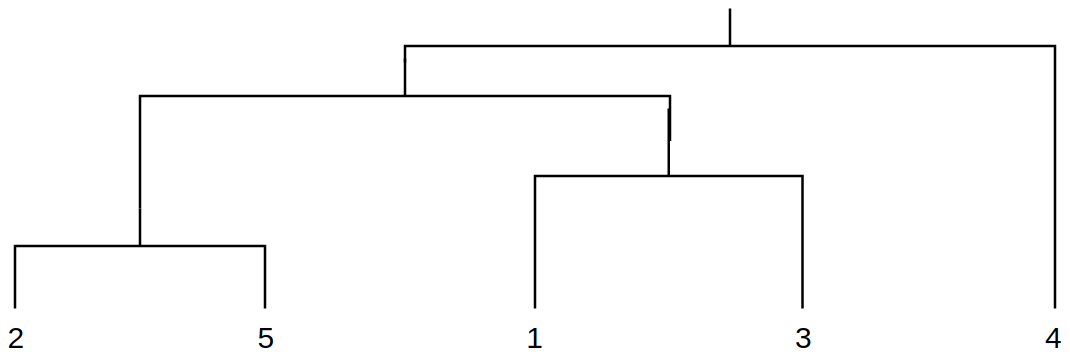
\includegraphics{./dendrogram01.png}
\caption{Dendrogram01}
\end{figure}

    \hypertarget{b}{%
\subsubsection{(b)}\label{b}}

Step 1. Combine 2 and 5

\begin{longtable}[]{@{}lcccc@{}}
\toprule
& 1 & 25 & 3 & 4\tabularnewline
\midrule
\endhead
1 & 0 & - & - & -\tabularnewline
25 & 0.3 & 0 & - & -\tabularnewline
3 & 0.4 & 0.4 & 0 & -\tabularnewline
4 & 0.7 & 0.35 & 0.45 & 0\tabularnewline
\bottomrule
\end{longtable}

Step 2. Combine 1 and 25

\begin{longtable}[]{@{}lccc@{}}
\toprule
& 125 & 3 & 4\tabularnewline
\midrule
\endhead
125 & 0 & - & -\tabularnewline
3 & 0.4 & 0 & -\tabularnewline
4 & 0.35 & 0.45 & 0\tabularnewline
\bottomrule
\end{longtable}

Step 3. Combine 125 and 4

\begin{longtable}[]{@{}lcc@{}}
\toprule
& 1254 & 3\tabularnewline
\midrule
\endhead
1254 & 0 & -\tabularnewline
3 & 0.4 & 0\tabularnewline
\bottomrule
\end{longtable}

Step 4. Combine 1254 and 3

\begin{longtable}[]{@{}lc@{}}
\toprule
& 12543\tabularnewline
\midrule
\endhead
12543 & 0\tabularnewline
\bottomrule
\end{longtable}

\begin{figure}
\centering
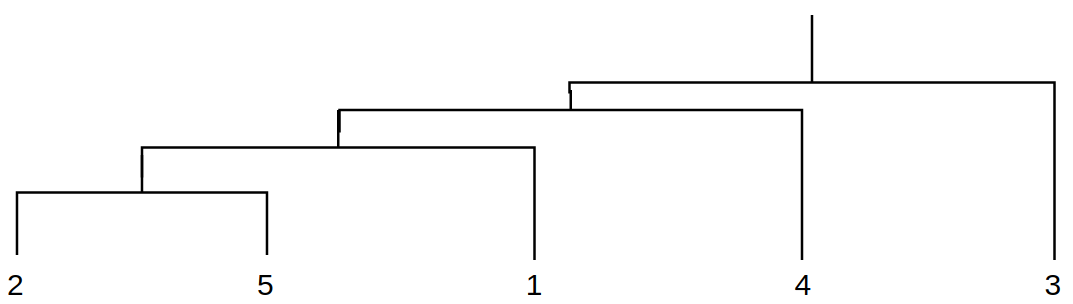
\includegraphics{./dendrogram02.png}
\caption{Dendrogram02}
\end{figure}

    \hypertarget{c}{%
\subsubsection{(c)}\label{c}}

Complete Linkage Clusters:

(2, 5), (1, 3), (4)

\begin{figure}
\centering
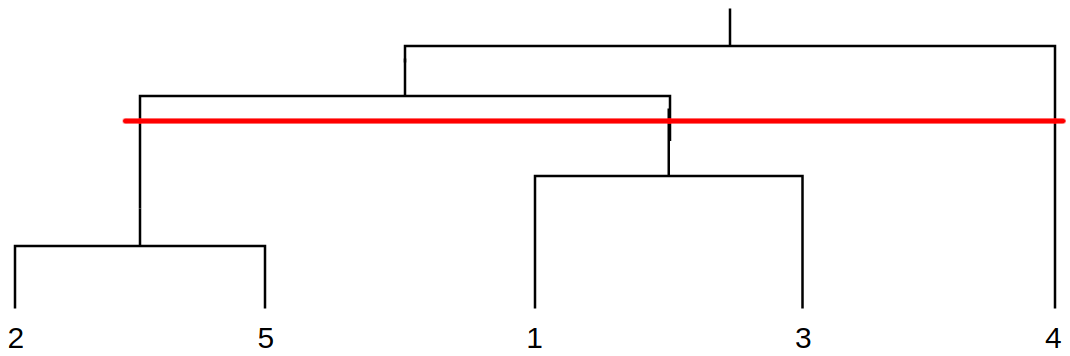
\includegraphics{./dendrogram01_cut.png}
\caption{Dendrogram01\_cut}
\end{figure}

Single Linkage Clusters:

(2, 5, 1), (4), (3)

\begin{figure}
\centering
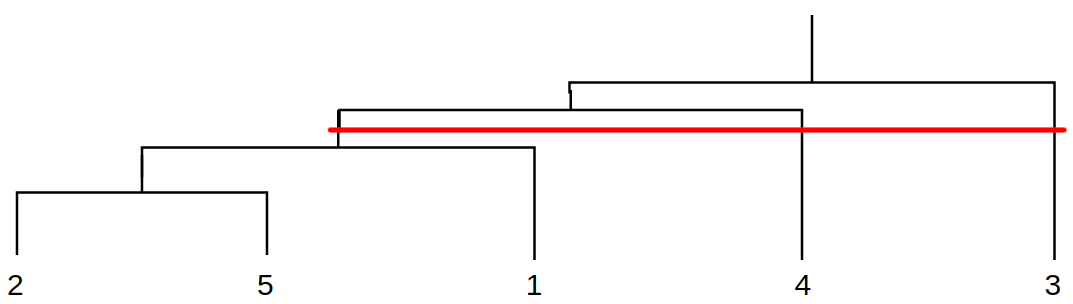
\includegraphics{./dendrogram02_cut.png}
\caption{Dendrogram02\_cut}
\end{figure}

    \hypertarget{part-b}{%
\section{Part B}\label{part-b}}

    \hypertarget{question-4}{%
\subsection{Question 4}\label{question-4}}

    \begin{tcolorbox}[breakable, size=fbox, boxrule=1pt, pad at break*=1mm,colback=cellbackground, colframe=cellborder]
\prompt{In}{incolor}{6}{\boxspacing}
\begin{Verbatim}[commandchars=\\\{\}]
\PY{n}{nums} \PY{o}{=} \PY{n}{np}\PY{o}{.}\PY{n}{array}\PY{p}{(}\PY{p}{[}\PY{l+m+mi}{20}\PY{p}{,}\PY{l+m+mi}{30}\PY{p}{,}\PY{l+m+mi}{40}\PY{p}{,}\PY{l+m+mi}{60}\PY{p}{,}\PY{l+m+mi}{120}\PY{p}{]}\PY{p}{)}\PY{o}{.}\PY{n}{reshape}\PY{p}{(}\PY{o}{\PYZhy{}}\PY{l+m+mi}{1}\PY{p}{,}\PY{l+m+mi}{1}\PY{p}{)}

\PY{n}{scaler} \PY{o}{=} \PY{n}{MinMaxScaler}\PY{p}{(}\PY{p}{)}
\PY{n}{ns1} \PY{o}{=} \PY{n}{scaler}\PY{o}{.}\PY{n}{fit\PYZus{}transform}\PY{p}{(}\PY{n}{nums}\PY{p}{)}
\PY{n}{scaler} \PY{o}{=} \PY{n}{MinMaxScaler}\PY{p}{(}\PY{p}{[}\PY{o}{\PYZhy{}}\PY{l+m+mi}{1}\PY{p}{,}\PY{l+m+mi}{1}\PY{p}{]}\PY{p}{)}
\PY{n}{ns2} \PY{o}{=} \PY{n}{scaler}\PY{o}{.}\PY{n}{fit\PYZus{}transform}\PY{p}{(}\PY{n}{nums}\PY{p}{)}
\PY{n}{scaler} \PY{o}{=} \PY{n}{StandardScaler}\PY{p}{(}\PY{p}{)}
\PY{n}{ns3} \PY{o}{=} \PY{n}{scaler}\PY{o}{.}\PY{n}{fit\PYZus{}transform}\PY{p}{(}\PY{n}{nums}\PY{p}{)}

\PY{n}{normed} \PY{o}{=} \PY{n}{pd}\PY{o}{.}\PY{n}{DataFrame}\PY{p}{(}\PY{p}{\PYZob{}}
    \PY{l+s+s2}{\PYZdq{}}\PY{l+s+s2}{orig}\PY{l+s+s2}{\PYZdq{}}\PY{p}{:} \PY{p}{[}\PY{l+m+mi}{20}\PY{p}{,}\PY{l+m+mi}{30}\PY{p}{,}\PY{l+m+mi}{40}\PY{p}{,}\PY{l+m+mi}{60}\PY{p}{,}\PY{l+m+mi}{120}\PY{p}{]}\PY{p}{,}
    \PY{l+s+s2}{\PYZdq{}}\PY{l+s+s2}{minMax}\PY{l+s+s2}{\PYZdq{}}\PY{p}{:} \PY{p}{[}\PY{n}{ns1}\PY{p}{[}\PY{l+m+mi}{0}\PY{p}{]}\PY{p}{[}\PY{l+m+mi}{0}\PY{p}{]}\PY{p}{,}\PY{n}{ns1}\PY{p}{[}\PY{l+m+mi}{1}\PY{p}{]}\PY{p}{[}\PY{l+m+mi}{0}\PY{p}{]}\PY{p}{,}\PY{n}{ns1}\PY{p}{[}\PY{l+m+mi}{2}\PY{p}{]}\PY{p}{[}\PY{l+m+mi}{0}\PY{p}{]}\PY{p}{,}\PY{n}{ns1}\PY{p}{[}\PY{l+m+mi}{3}\PY{p}{]}\PY{p}{[}\PY{l+m+mi}{0}\PY{p}{]}\PY{p}{,}\PY{n}{ns1}\PY{p}{[}\PY{l+m+mi}{4}\PY{p}{]}\PY{p}{[}\PY{l+m+mi}{0}\PY{p}{]}\PY{p}{]}\PY{p}{,}
    \PY{l+s+s2}{\PYZdq{}}\PY{l+s+s2}{minMaxNeg}\PY{l+s+s2}{\PYZdq{}}\PY{p}{:} \PY{p}{[}\PY{n}{ns2}\PY{p}{[}\PY{l+m+mi}{0}\PY{p}{]}\PY{p}{[}\PY{l+m+mi}{0}\PY{p}{]}\PY{p}{,}\PY{n}{ns2}\PY{p}{[}\PY{l+m+mi}{1}\PY{p}{]}\PY{p}{[}\PY{l+m+mi}{0}\PY{p}{]}\PY{p}{,}\PY{n}{ns2}\PY{p}{[}\PY{l+m+mi}{2}\PY{p}{]}\PY{p}{[}\PY{l+m+mi}{0}\PY{p}{]}\PY{p}{,}\PY{n}{ns2}\PY{p}{[}\PY{l+m+mi}{3}\PY{p}{]}\PY{p}{[}\PY{l+m+mi}{0}\PY{p}{]}\PY{p}{,}\PY{n}{ns2}\PY{p}{[}\PY{l+m+mi}{4}\PY{p}{]}\PY{p}{[}\PY{l+m+mi}{0}\PY{p}{]}\PY{p}{]}\PY{p}{,}
    \PY{l+s+s2}{\PYZdq{}}\PY{l+s+s2}{z\PYZhy{}score}\PY{l+s+s2}{\PYZdq{}}\PY{p}{:} \PY{p}{[}\PY{n}{ns3}\PY{p}{[}\PY{l+m+mi}{0}\PY{p}{]}\PY{p}{[}\PY{l+m+mi}{0}\PY{p}{]}\PY{p}{,}\PY{n}{ns3}\PY{p}{[}\PY{l+m+mi}{1}\PY{p}{]}\PY{p}{[}\PY{l+m+mi}{0}\PY{p}{]}\PY{p}{,}\PY{n}{ns3}\PY{p}{[}\PY{l+m+mi}{2}\PY{p}{]}\PY{p}{[}\PY{l+m+mi}{0}\PY{p}{]}\PY{p}{,}\PY{n}{ns3}\PY{p}{[}\PY{l+m+mi}{3}\PY{p}{]}\PY{p}{[}\PY{l+m+mi}{0}\PY{p}{]}\PY{p}{,}\PY{n}{ns3}\PY{p}{[}\PY{l+m+mi}{4}\PY{p}{]}\PY{p}{[}\PY{l+m+mi}{0}\PY{p}{]}\PY{p}{]} 
\PY{p}{\PYZcb{}}\PY{p}{)}

\PY{n+nb}{print}\PY{p}{(}\PY{l+s+s2}{\PYZdq{}}\PY{l+s+s2}{Normalized vectors}\PY{l+s+s2}{\PYZdq{}}\PY{p}{)}
\PY{n}{display}\PY{p}{(}\PY{n}{normed}\PY{p}{)}
\end{Verbatim}
\end{tcolorbox}

    \begin{Verbatim}[commandchars=\\\{\}]
Normalized vectors
    \end{Verbatim}

    
    \begin{Verbatim}[commandchars=\\\{\}]
   orig  minMax  minMaxNeg   z-score
0    20     0.0       -1.0 -0.956325
1    30     0.1       -0.8 -0.675053
2    40     0.2       -0.6 -0.393781
3    60     0.4       -0.2  0.168763
4   120     1.0        1.0  1.856395
    \end{Verbatim}

    
    \hypertarget{question-5}{%
\subsection{Question 5}\label{question-5}}

    \hypertarget{a}{%
\subsubsection{(a)}\label{a}}

    \begin{tcolorbox}[breakable, size=fbox, boxrule=1pt, pad at break*=1mm,colback=cellbackground, colframe=cellborder]
\prompt{In}{incolor}{7}{\boxspacing}
\begin{Verbatim}[commandchars=\\\{\}]
\PY{n}{samples} \PY{o}{=} \PY{n}{pd}\PY{o}{.}\PY{n}{DataFrame}\PY{p}{(}\PY{p}{\PYZob{}}
    \PY{l+s+s2}{\PYZdq{}}\PY{l+s+s2}{A}\PY{l+s+s2}{\PYZdq{}}\PY{p}{:} \PY{p}{[}\PY{l+m+mf}{1.4}\PY{p}{,}\PY{l+m+mf}{1.8}\PY{p}{,}\PY{l+m+mf}{1.3}\PY{p}{,}\PY{l+m+mf}{0.9}\PY{p}{,}\PY{l+m+mf}{1.5}\PY{p}{]}\PY{p}{,}
    \PY{l+s+s2}{\PYZdq{}}\PY{l+s+s2}{B}\PY{l+s+s2}{\PYZdq{}}\PY{p}{:} \PY{p}{[}\PY{l+m+mf}{1.3}\PY{p}{,}\PY{l+m+mf}{1.1}\PY{p}{,}\PY{l+m+mf}{1.2}\PY{p}{,}\PY{l+m+mf}{3.3}\PY{p}{,}\PY{l+m+mf}{2.1}\PY{p}{]}\PY{p}{,}
    \PY{l+s+s2}{\PYZdq{}}\PY{l+s+s2}{C}\PY{l+s+s2}{\PYZdq{}}\PY{p}{:} \PY{p}{[}\PY{l+m+mf}{2.9}\PY{p}{,}\PY{l+m+mf}{3.2}\PY{p}{,}\PY{l+m+mf}{2.9}\PY{p}{,}\PY{l+m+mf}{3.1}\PY{p}{,}\PY{l+m+mf}{3.3}\PY{p}{]}
\PY{p}{\PYZcb{}}\PY{p}{)}

\PY{n}{distances} \PY{o}{=} \PY{n}{pd}\PY{o}{.}\PY{n}{DataFrame}\PY{p}{(}\PY{p}{\PYZob{}}
    \PY{l+s+s2}{\PYZdq{}}\PY{l+s+s2}{sample}\PY{l+s+s2}{\PYZdq{}}\PY{p}{:} \PY{p}{[}\PY{l+s+s2}{\PYZdq{}}\PY{l+s+s2}{x1}\PY{l+s+s2}{\PYZdq{}}\PY{p}{,}\PY{l+s+s2}{\PYZdq{}}\PY{l+s+s2}{x2}\PY{l+s+s2}{\PYZdq{}}\PY{p}{,}\PY{l+s+s2}{\PYZdq{}}\PY{l+s+s2}{x3}\PY{l+s+s2}{\PYZdq{}}\PY{p}{,}\PY{l+s+s2}{\PYZdq{}}\PY{l+s+s2}{x4}\PY{l+s+s2}{\PYZdq{}}\PY{p}{,}\PY{l+s+s2}{\PYZdq{}}\PY{l+s+s2}{x5}\PY{l+s+s2}{\PYZdq{}}\PY{p}{]}\PY{p}{,}
    \PY{l+s+s2}{\PYZdq{}}\PY{l+s+s2}{man}\PY{l+s+s2}{\PYZdq{}}\PY{p}{:} \PY{p}{[}\PY{l+m+mf}{0.}\PY{p}{,}\PY{l+m+mf}{0.}\PY{p}{,}\PY{l+m+mf}{0.}\PY{p}{,}\PY{l+m+mf}{0.}\PY{p}{,}\PY{l+m+mf}{0.}\PY{p}{]}\PY{p}{,}
    \PY{l+s+s2}{\PYZdq{}}\PY{l+s+s2}{euc}\PY{l+s+s2}{\PYZdq{}}\PY{p}{:} \PY{p}{[}\PY{l+m+mf}{0.}\PY{p}{,}\PY{l+m+mf}{0.}\PY{p}{,}\PY{l+m+mf}{0.}\PY{p}{,}\PY{l+m+mf}{0.}\PY{p}{,}\PY{l+m+mf}{0.}\PY{p}{]}\PY{p}{,}
    \PY{l+s+s2}{\PYZdq{}}\PY{l+s+s2}{min}\PY{l+s+s2}{\PYZdq{}}\PY{p}{:} \PY{p}{[}\PY{l+m+mf}{0.}\PY{p}{,}\PY{l+m+mf}{0.}\PY{p}{,}\PY{l+m+mf}{0.}\PY{p}{,}\PY{l+m+mf}{0.}\PY{p}{,}\PY{l+m+mf}{0.}\PY{p}{]}\PY{p}{,}
    \PY{l+s+s2}{\PYZdq{}}\PY{l+s+s2}{sup}\PY{l+s+s2}{\PYZdq{}}\PY{p}{:} \PY{p}{[}\PY{l+m+mf}{0.}\PY{p}{,}\PY{l+m+mf}{0.}\PY{p}{,}\PY{l+m+mf}{0.}\PY{p}{,}\PY{l+m+mf}{0.}\PY{p}{,}\PY{l+m+mf}{0.}\PY{p}{]}\PY{p}{,}
    \PY{l+s+s2}{\PYZdq{}}\PY{l+s+s2}{cos}\PY{l+s+s2}{\PYZdq{}}\PY{p}{:} \PY{p}{[}\PY{l+m+mf}{0.}\PY{p}{,}\PY{l+m+mf}{0.}\PY{p}{,}\PY{l+m+mf}{0.}\PY{p}{,}\PY{l+m+mf}{0.}\PY{p}{,}\PY{l+m+mf}{0.}\PY{p}{]}
\PY{p}{\PYZcb{}}\PY{p}{)}

\PY{n}{newP} \PY{o}{=} \PY{p}{[}\PY{l+m+mf}{1.25}\PY{p}{,}\PY{l+m+mf}{1.74}\PY{p}{,}\PY{l+m+mf}{3.01}\PY{p}{]}

\PY{k}{for} \PY{n}{index}\PY{p}{,} \PY{n}{row} \PY{o+ow}{in} \PY{n}{samples}\PY{o}{.}\PY{n}{iterrows}\PY{p}{(}\PY{p}{)}\PY{p}{:}
    \PY{n}{distances}\PY{o}{.}\PY{n}{at}\PY{p}{[}\PY{n}{index}\PY{p}{,}\PY{l+s+s2}{\PYZdq{}}\PY{l+s+s2}{man}\PY{l+s+s2}{\PYZdq{}}\PY{p}{]} \PY{o}{=} \PY{n+nb}{abs}\PY{p}{(}\PY{n}{newP}\PY{p}{[}\PY{l+m+mi}{0}\PY{p}{]}\PY{o}{\PYZhy{}}\PY{n}{row}\PY{p}{[}\PY{l+m+mi}{0}\PY{p}{]}\PY{p}{)} \PY{o}{+} \PY{n+nb}{abs}\PY{p}{(}\PY{n}{newP}\PY{p}{[}\PY{l+m+mi}{1}\PY{p}{]}\PY{o}{\PYZhy{}}\PY{n}{row}\PY{p}{[}\PY{l+m+mi}{1}\PY{p}{]}\PY{p}{)} \PY{o}{+} \PY{n+nb}{abs}\PY{p}{(}\PY{n}{newP}\PY{p}{[}\PY{l+m+mi}{2}\PY{p}{]}\PY{o}{\PYZhy{}}\PY{n}{row}\PY{p}{[}\PY{l+m+mi}{2}\PY{p}{]}\PY{p}{)}
    \PY{n}{distances}\PY{o}{.}\PY{n}{at}\PY{p}{[}\PY{n}{index}\PY{p}{,}\PY{l+s+s2}{\PYZdq{}}\PY{l+s+s2}{euc}\PY{l+s+s2}{\PYZdq{}}\PY{p}{]} \PY{o}{=} \PY{n}{np}\PY{o}{.}\PY{n}{linalg}\PY{o}{.}\PY{n}{norm}\PY{p}{(}\PY{n}{newP}\PY{o}{\PYZhy{}}\PY{n}{row}\PY{p}{)}
    \PY{n}{distances}\PY{o}{.}\PY{n}{at}\PY{p}{[}\PY{n}{index}\PY{p}{,}\PY{l+s+s2}{\PYZdq{}}\PY{l+s+s2}{min}\PY{l+s+s2}{\PYZdq{}}\PY{p}{]} \PY{o}{=} \PY{n}{distance}\PY{o}{.}\PY{n}{minkowski}\PY{p}{(}\PY{n}{newP}\PY{p}{,} \PY{n}{row}\PY{p}{,} \PY{l+m+mi}{3}\PY{p}{)}
    \PY{n}{distances}\PY{o}{.}\PY{n}{at}\PY{p}{[}\PY{n}{index}\PY{p}{,}\PY{l+s+s2}{\PYZdq{}}\PY{l+s+s2}{sup}\PY{l+s+s2}{\PYZdq{}}\PY{p}{]} \PY{o}{=} \PY{n}{distance}\PY{o}{.}\PY{n}{chebyshev}\PY{p}{(}\PY{n}{newP}\PY{p}{,} \PY{n}{row}\PY{p}{)}
    \PY{n}{distances}\PY{o}{.}\PY{n}{at}\PY{p}{[}\PY{n}{index}\PY{p}{,}\PY{l+s+s2}{\PYZdq{}}\PY{l+s+s2}{cos}\PY{l+s+s2}{\PYZdq{}}\PY{p}{]} \PY{o}{=} \PY{n}{distance}\PY{o}{.}\PY{n}{cosine}\PY{p}{(}\PY{n}{newP}\PY{p}{,} \PY{n}{row}\PY{p}{)}

\PY{n+nb}{print}\PY{p}{(}\PY{l+s+s2}{\PYZdq{}}\PY{l+s+s2}{Distances from new point to data points}\PY{l+s+s2}{\PYZdq{}}\PY{p}{)}
\PY{n}{display}\PY{p}{(}\PY{n}{distances}\PY{p}{)}
\end{Verbatim}
\end{tcolorbox}

    \begin{Verbatim}[commandchars=\\\{\}]
Distances from new point to data points
    \end{Verbatim}

    
    \begin{Verbatim}[commandchars=\\\{\}]
  sample   man       euc       min   sup       cos
0     x1  0.70  0.477703  0.447958  0.44  0.006975
1     x2  1.38  0.864986  0.757918  0.64  0.025745
2     x3  0.70  0.553353  0.541659  0.54  0.008671
3     x4  2.00  1.601312  1.565950  1.56  0.050270
4     x5  0.90  0.525547  0.442544  0.36  0.001018
    \end{Verbatim}

    
    \hypertarget{b}{%
\subsubsection{(b)}\label{b}}

    \begin{tcolorbox}[breakable, size=fbox, boxrule=1pt, pad at break*=1mm,colback=cellbackground, colframe=cellborder]
\prompt{In}{incolor}{8}{\boxspacing}
\begin{Verbatim}[commandchars=\\\{\}]
\PY{n}{arrSamples} \PY{o}{=} \PY{n}{samples}\PY{o}{.}\PY{n}{values}
\PY{n}{arrNewP} \PY{o}{=} \PY{n}{np}\PY{o}{.}\PY{n}{array}\PY{p}{(}\PY{n}{newP}\PY{p}{)}\PY{o}{.}\PY{n}{reshape}\PY{p}{(}\PY{l+m+mi}{1}\PY{p}{,}\PY{o}{\PYZhy{}}\PY{l+m+mi}{1}\PY{p}{)}

\PY{n}{scaler} \PY{o}{=} \PY{n}{MinMaxScaler}\PY{p}{(}\PY{p}{)}
\PY{n}{scaler}\PY{o}{.}\PY{n}{fit}\PY{p}{(}\PY{n}{arrSamples}\PY{p}{)}

\PY{n}{normSamples} \PY{o}{=} \PY{n}{scaler}\PY{o}{.}\PY{n}{transform}\PY{p}{(}\PY{n}{arrSamples}\PY{p}{)}
\PY{n}{normSamples} \PY{o}{=} \PY{n}{pd}\PY{o}{.}\PY{n}{DataFrame}\PY{p}{(}\PY{n}{data}\PY{o}{=}\PY{n}{normSamples}\PY{p}{)}

\PY{n}{normNewP} \PY{o}{=} \PY{n}{scaler}\PY{o}{.}\PY{n}{transform}\PY{p}{(}\PY{n}{arrNewP}\PY{p}{)}\PY{p}{[}\PY{l+m+mi}{0}\PY{p}{]}

\PY{n}{normDistances} \PY{o}{=} \PY{n}{pd}\PY{o}{.}\PY{n}{DataFrame}\PY{p}{(}\PY{p}{\PYZob{}}
    \PY{l+s+s2}{\PYZdq{}}\PY{l+s+s2}{sample}\PY{l+s+s2}{\PYZdq{}}\PY{p}{:} \PY{p}{[}\PY{l+s+s2}{\PYZdq{}}\PY{l+s+s2}{x1}\PY{l+s+s2}{\PYZdq{}}\PY{p}{,}\PY{l+s+s2}{\PYZdq{}}\PY{l+s+s2}{x2}\PY{l+s+s2}{\PYZdq{}}\PY{p}{,}\PY{l+s+s2}{\PYZdq{}}\PY{l+s+s2}{x3}\PY{l+s+s2}{\PYZdq{}}\PY{p}{,}\PY{l+s+s2}{\PYZdq{}}\PY{l+s+s2}{x4}\PY{l+s+s2}{\PYZdq{}}\PY{p}{,}\PY{l+s+s2}{\PYZdq{}}\PY{l+s+s2}{x5}\PY{l+s+s2}{\PYZdq{}}\PY{p}{]}\PY{p}{,}
    \PY{l+s+s2}{\PYZdq{}}\PY{l+s+s2}{euc}\PY{l+s+s2}{\PYZdq{}}\PY{p}{:} \PY{p}{[}\PY{l+m+mf}{0.}\PY{p}{,}\PY{l+m+mf}{0.}\PY{p}{,}\PY{l+m+mf}{0.}\PY{p}{,}\PY{l+m+mf}{0.}\PY{p}{,}\PY{l+m+mf}{0.}\PY{p}{]}
\PY{p}{\PYZcb{}}\PY{p}{)}
\PY{k}{for} \PY{n}{index}\PY{p}{,} \PY{n}{row} \PY{o+ow}{in} \PY{n}{normSamples}\PY{o}{.}\PY{n}{iterrows}\PY{p}{(}\PY{p}{)}\PY{p}{:}
    \PY{n}{normDistances}\PY{o}{.}\PY{n}{at}\PY{p}{[}\PY{n}{index}\PY{p}{,}\PY{l+s+s2}{\PYZdq{}}\PY{l+s+s2}{euc}\PY{l+s+s2}{\PYZdq{}}\PY{p}{]} \PY{o}{=} \PY{n}{np}\PY{o}{.}\PY{n}{linalg}\PY{o}{.}\PY{n}{norm}\PY{p}{(}\PY{n}{normNewP}\PY{o}{\PYZhy{}}\PY{n}{row}\PY{p}{)}

\PY{n+nb}{print}\PY{p}{(}\PY{l+s+s2}{\PYZdq{}}\PY{l+s+s2}{Euclidean Distances with Normalization}\PY{l+s+s2}{\PYZdq{}}\PY{p}{)}
\PY{n}{display}\PY{p}{(}\PY{n}{normDistances}\PY{p}{)}
\end{Verbatim}
\end{tcolorbox}

    \begin{Verbatim}[commandchars=\\\{\}]
Euclidean Distances with Normalization
    \end{Verbatim}

    
    \begin{Verbatim}[commandchars=\\\{\}]
  sample       euc
0     x1  0.378686
1     x2  0.826868
2     x3  0.372773
3     x4  0.839446
4     x5  0.793450
    \end{Verbatim}

    
    \hypertarget{question-6}{%
\subsection{Question 6}\label{question-6}}

    \hypertarget{a}{%
\subsubsection{(a)}\label{a}}

    \begin{tcolorbox}[breakable, size=fbox, boxrule=1pt, pad at break*=1mm,colback=cellbackground, colframe=cellborder]
\prompt{In}{incolor}{9}{\boxspacing}
\begin{Verbatim}[commandchars=\\\{\}]
\PY{n}{pokemon} \PY{o}{=} \PY{n}{pd}\PY{o}{.}\PY{n}{read\PYZus{}csv}\PY{p}{(}\PY{l+s+s2}{\PYZdq{}}\PY{l+s+s2}{Pokemon.csv}\PY{l+s+s2}{\PYZdq{}}\PY{p}{,} \PY{n}{sep}\PY{o}{=}\PY{l+s+s2}{\PYZdq{}}\PY{l+s+s2}{,}\PY{l+s+s2}{\PYZdq{}}\PY{p}{,} \PY{n}{engine}\PY{o}{=}\PY{l+s+s2}{\PYZdq{}}\PY{l+s+s2}{python}\PY{l+s+s2}{\PYZdq{}}\PY{p}{)}
\PY{n}{stats} \PY{o}{=} \PY{p}{[}\PY{l+s+s2}{\PYZdq{}}\PY{l+s+s2}{HP}\PY{l+s+s2}{\PYZdq{}}\PY{p}{,}\PY{l+s+s2}{\PYZdq{}}\PY{l+s+s2}{Attack}\PY{l+s+s2}{\PYZdq{}}\PY{p}{,}\PY{l+s+s2}{\PYZdq{}}\PY{l+s+s2}{Defense}\PY{l+s+s2}{\PYZdq{}}\PY{p}{,}\PY{l+s+s2}{\PYZdq{}}\PY{l+s+s2}{SpAtk}\PY{l+s+s2}{\PYZdq{}}\PY{p}{,}\PY{l+s+s2}{\PYZdq{}}\PY{l+s+s2}{SpDef}\PY{l+s+s2}{\PYZdq{}}\PY{p}{,}\PY{l+s+s2}{\PYZdq{}}\PY{l+s+s2}{Speed}\PY{l+s+s2}{\PYZdq{}}\PY{p}{]}
\PY{n}{plot} \PY{o}{=} \PY{n}{sb}\PY{o}{.}\PY{n}{boxplot}\PY{p}{(}\PY{n}{x}\PY{o}{=}\PY{l+s+s2}{\PYZdq{}}\PY{l+s+s2}{variable}\PY{l+s+s2}{\PYZdq{}}\PY{p}{,} \PY{n}{y}\PY{o}{=}\PY{l+s+s2}{\PYZdq{}}\PY{l+s+s2}{value}\PY{l+s+s2}{\PYZdq{}}\PY{p}{,} \PY{n}{data}\PY{o}{=}\PY{n}{pd}\PY{o}{.}\PY{n}{melt}\PY{p}{(}\PY{n}{pokemon}\PY{p}{[}\PY{n}{stats}\PY{p}{]}\PY{p}{)}\PY{p}{)}
\PY{n}{plot}\PY{o}{.}\PY{n}{set}\PY{p}{(}\PY{n}{xlabel}\PY{o}{=}\PY{l+s+s2}{\PYZdq{}}\PY{l+s+s2}{Stat}\PY{l+s+s2}{\PYZdq{}}\PY{p}{,} \PY{n}{ylabel}\PY{o}{=}\PY{l+s+s2}{\PYZdq{}}\PY{l+s+s2}{Value}\PY{l+s+s2}{\PYZdq{}}\PY{p}{)}
\PY{n}{plot}\PY{o}{.}\PY{n}{set\PYZus{}title}\PY{p}{(}\PY{l+s+s2}{\PYZdq{}}\PY{l+s+s2}{Pokemon Stat Spread}\PY{l+s+s2}{\PYZdq{}}\PY{p}{)}
\PY{n}{plt}\PY{o}{.}\PY{n}{show}\PY{p}{(}\PY{p}{)}
\end{Verbatim}
\end{tcolorbox}

    \begin{center}
    \adjustimage{max size={0.9\linewidth}{0.9\paperheight}}{P2_Grant_Eric_files/P2_Grant_Eric_27_0.pdf}
    \end{center}
    { \hspace*{\fill} \\}
    
    \hypertarget{b}{%
\subsubsection{(b)}\label{b}}

    \begin{tcolorbox}[breakable, size=fbox, boxrule=1pt, pad at break*=1mm,colback=cellbackground, colframe=cellborder]
\prompt{In}{incolor}{10}{\boxspacing}
\begin{Verbatim}[commandchars=\\\{\}]
\PY{n}{scaler} \PY{o}{=} \PY{n}{MinMaxScaler}\PY{p}{(}\PY{p}{)}
\PY{n}{scaler}\PY{o}{.}\PY{n}{fit}\PY{p}{(}\PY{n}{pokemon}\PY{p}{[}\PY{n}{stats}\PY{p}{]}\PY{p}{)}
\PY{n}{pokemon}\PY{p}{[}\PY{n}{stats}\PY{p}{]} \PY{o}{=} \PY{n}{scaler}\PY{o}{.}\PY{n}{transform}\PY{p}{(}\PY{n}{pokemon}\PY{p}{[}\PY{n}{stats}\PY{p}{]}\PY{p}{)}

\PY{n}{plot} \PY{o}{=} \PY{n}{sb}\PY{o}{.}\PY{n}{boxplot}\PY{p}{(}\PY{n}{x}\PY{o}{=}\PY{l+s+s2}{\PYZdq{}}\PY{l+s+s2}{variable}\PY{l+s+s2}{\PYZdq{}}\PY{p}{,} \PY{n}{y}\PY{o}{=}\PY{l+s+s2}{\PYZdq{}}\PY{l+s+s2}{value}\PY{l+s+s2}{\PYZdq{}}\PY{p}{,} \PY{n}{data}\PY{o}{=}\PY{n}{pd}\PY{o}{.}\PY{n}{melt}\PY{p}{(}\PY{n}{pokemon}\PY{p}{[}\PY{n}{stats}\PY{p}{]}\PY{p}{)}\PY{p}{)}
\PY{n}{plot}\PY{o}{.}\PY{n}{set}\PY{p}{(}\PY{n}{xlabel}\PY{o}{=}\PY{l+s+s2}{\PYZdq{}}\PY{l+s+s2}{Stat}\PY{l+s+s2}{\PYZdq{}}\PY{p}{,} \PY{n}{ylabel}\PY{o}{=}\PY{l+s+s2}{\PYZdq{}}\PY{l+s+s2}{Value}\PY{l+s+s2}{\PYZdq{}}\PY{p}{)}
\PY{n}{plot}\PY{o}{.}\PY{n}{set\PYZus{}title}\PY{p}{(}\PY{l+s+s2}{\PYZdq{}}\PY{l+s+s2}{Pokemon Stat Spread Normalized}\PY{l+s+s2}{\PYZdq{}}\PY{p}{)}
\PY{n}{plt}\PY{o}{.}\PY{n}{show}\PY{p}{(}\PY{p}{)}
\end{Verbatim}
\end{tcolorbox}

    \begin{center}
    \adjustimage{max size={0.9\linewidth}{0.9\paperheight}}{P2_Grant_Eric_files/P2_Grant_Eric_29_0.pdf}
    \end{center}
    { \hspace*{\fill} \\}
    
    \hypertarget{c}{%
\subsubsection{(c)}\label{c}}

    \begin{tcolorbox}[breakable, size=fbox, boxrule=1pt, pad at break*=1mm,colback=cellbackground, colframe=cellborder]
\prompt{In}{incolor}{11}{\boxspacing}
\begin{Verbatim}[commandchars=\\\{\}]
\PY{n}{kClusters} \PY{o}{=} \PY{p}{[}\PY{p}{]}
\PY{k}{for} \PY{n}{n} \PY{o+ow}{in} \PY{n+nb}{range}\PY{p}{(}\PY{l+m+mi}{3}\PY{p}{,}\PY{l+m+mi}{9}\PY{p}{)}\PY{p}{:}
    \PY{n}{kmeans} \PY{o}{=} \PY{n}{cluster}\PY{o}{.}\PY{n}{KMeans}\PY{p}{(}\PY{n}{n\PYZus{}clusters}\PY{o}{=}\PY{n}{n}\PY{p}{)}\PY{o}{.}\PY{n}{fit}\PY{p}{(}\PY{n}{pokemon}\PY{p}{[}\PY{n}{stats}\PY{p}{]}\PY{p}{)}
    \PY{n}{kClusters}\PY{o}{.}\PY{n}{append}\PY{p}{(}\PY{n}{kmeans}\PY{o}{.}\PY{n}{cluster\PYZus{}centers\PYZus{}}\PY{p}{)}
\end{Verbatim}
\end{tcolorbox}

    \hypertarget{d}{%
\subsubsection{(d)}\label{d}}

    \begin{tcolorbox}[breakable, size=fbox, boxrule=1pt, pad at break*=1mm,colback=cellbackground, colframe=cellborder]
\prompt{In}{incolor}{12}{\boxspacing}
\begin{Verbatim}[commandchars=\\\{\}]
\PY{n}{k}\PY{p}{,} \PY{n}{labels} \PY{o}{=} \PY{n}{gs}\PY{o}{.}\PY{n}{gapstat}\PY{p}{(}\PY{n}{pokemon}\PY{p}{[}\PY{n}{stats}\PY{p}{]}\PY{p}{)}
\PY{n+nb}{print}\PY{p}{(}\PY{l+s+s2}{\PYZdq{}}\PY{l+s+s2}{Optimal number of clusters:}\PY{l+s+s2}{\PYZdq{}}\PY{p}{,}\PY{n}{k}\PY{p}{)}
\end{Verbatim}
\end{tcolorbox}

    \begin{Verbatim}[commandchars=\\\{\}]
Optimal number of clusters: 4
    \end{Verbatim}

    \hypertarget{e}{%
\subsubsection{(e)}\label{e}}

    \begin{tcolorbox}[breakable, size=fbox, boxrule=1pt, pad at break*=1mm,colback=cellbackground, colframe=cellborder]
\prompt{In}{incolor}{13}{\boxspacing}
\begin{Verbatim}[commandchars=\\\{\}]
\PY{n}{statCentroids} \PY{o}{=} \PY{n}{pd}\PY{o}{.}\PY{n}{DataFrame}\PY{p}{(}\PY{n}{data}\PY{o}{=}\PY{n}{kClusters}\PY{p}{[}\PY{n}{k}\PY{o}{\PYZhy{}}\PY{l+m+mi}{3}\PY{p}{]}\PY{p}{,} \PY{n}{columns}\PY{o}{=}\PY{n}{stats}\PY{p}{)}
\PY{n}{display}\PY{p}{(}\PY{n}{statCentroids}\PY{p}{)}
\end{Verbatim}
\end{tcolorbox}

    
    \begin{Verbatim}[commandchars=\\\{\}]
         HP    Attack   Defense     SpAtk     SpDef     Speed
0  0.344436  0.630041  0.380413  0.608407  0.361188  0.543919
1  0.305436  0.498948  0.454105  0.297937  0.308611  0.287938
2  0.203529  0.264016  0.211771  0.207876  0.145214  0.250141
3  0.288217  0.388237  0.281508  0.412852  0.276757  0.468848
    \end{Verbatim}

    
    \hypertarget{f}{%
\subsubsection{(f)}\label{f}}

    \begin{tcolorbox}[breakable, size=fbox, boxrule=1pt, pad at break*=1mm,colback=cellbackground, colframe=cellborder]
\prompt{In}{incolor}{14}{\boxspacing}
\begin{Verbatim}[commandchars=\\\{\}]
\PY{n}{orig} \PY{o}{=} \PY{n}{scaler}\PY{o}{.}\PY{n}{inverse\PYZus{}transform}\PY{p}{(}\PY{n}{statCentroids}\PY{p}{[}\PY{n}{stats}\PY{p}{]}\PY{p}{)}
\PY{n}{statCentroidsOrig} \PY{o}{=} \PY{n}{pd}\PY{o}{.}\PY{n}{DataFrame}\PY{p}{(}\PY{n}{data}\PY{o}{=}\PY{n}{orig}\PY{p}{,} \PY{n}{columns}\PY{o}{=}\PY{n}{stats}\PY{p}{)}
\PY{n}{display}\PY{p}{(}\PY{n}{statCentroidsOrig}\PY{p}{)}
\end{Verbatim}
\end{tcolorbox}

    
    \begin{Verbatim}[commandchars=\\\{\}]
          HP      Attack     Defense       SpAtk      SpDef       Speed
0  88.486726  121.557522   90.592920  121.946903  95.849558  100.185841
1  78.580838   97.305389  107.173653   64.820359  84.808383   55.389222
2  52.696246   53.843003   52.648464   48.249147  50.494881   48.774744
3  74.207048   76.823789   68.339207   85.964758  78.118943   87.048458
    \end{Verbatim}

    
    \hypertarget{g}{%
\subsubsection{(g)}\label{g}}

    \begin{tcolorbox}[breakable, size=fbox, boxrule=1pt, pad at break*=1mm,colback=cellbackground, colframe=cellborder]
\prompt{In}{incolor}{20}{\boxspacing}
\begin{Verbatim}[commandchars=\\\{\}]
\PY{n}{fig} \PY{o}{=} \PY{n}{go}\PY{o}{.}\PY{n}{Figure}\PY{p}{(}\PY{p}{)}
\PY{k}{for} \PY{n}{n} \PY{o+ow}{in} \PY{n+nb}{range}\PY{p}{(}\PY{l+m+mi}{0}\PY{p}{,}\PY{n}{k}\PY{p}{)}\PY{p}{:}   
    \PY{n}{gName} \PY{o}{=} \PY{l+s+s2}{\PYZdq{}}\PY{l+s+s2}{Group}\PY{l+s+s2}{\PYZdq{}} \PY{o}{+} \PY{n+nb}{str}\PY{p}{(}\PY{n}{n}\PY{o}{+}\PY{l+m+mi}{1}\PY{p}{)} 
    \PY{n}{fig}\PY{o}{.}\PY{n}{add\PYZus{}trace}\PY{p}{(}\PY{n}{go}\PY{o}{.}\PY{n}{Scatterpolar}\PY{p}{(}
        \PY{n}{r}\PY{o}{=}\PY{n}{statCentroidsOrig}\PY{o}{.}\PY{n}{iloc}\PY{p}{[}\PY{n}{n}\PY{p}{]}\PY{p}{,}
        \PY{n}{theta}\PY{o}{=}\PY{n}{stats}\PY{p}{,}
        \PY{n}{fill}\PY{o}{=}\PY{l+s+s2}{\PYZdq{}}\PY{l+s+s2}{toself}\PY{l+s+s2}{\PYZdq{}}\PY{p}{,}
        \PY{n}{name}\PY{o}{=}\PY{n}{gName}
    \PY{p}{)}\PY{p}{)}
\PY{n}{fig}\PY{o}{.}\PY{n}{show}\PY{p}{(}\PY{p}{)}
\end{Verbatim}
\end{tcolorbox}

    
    
    \hypertarget{question-7}{%
\subsection{Question 7}\label{question-7}}

    \begin{tcolorbox}[breakable, size=fbox, boxrule=1pt, pad at break*=1mm,colback=cellbackground, colframe=cellborder]
\prompt{In}{incolor}{16}{\boxspacing}
\begin{Verbatim}[commandchars=\\\{\}]
\PY{n}{music} \PY{o}{=} \PY{n}{pd}\PY{o}{.}\PY{n}{read\PYZus{}csv}\PY{p}{(}\PY{l+s+s2}{\PYZdq{}}\PY{l+s+s2}{music2.csv}\PY{l+s+s2}{\PYZdq{}}\PY{p}{,} \PY{n}{sep}\PY{o}{=}\PY{l+s+s2}{\PYZdq{}}\PY{l+s+s2}{,}\PY{l+s+s2}{\PYZdq{}}\PY{p}{,} \PY{n}{engine}\PY{o}{=}\PY{l+s+s2}{\PYZdq{}}\PY{l+s+s2}{python}\PY{l+s+s2}{\PYZdq{}}\PY{p}{)}
\PY{n}{vals} \PY{o}{=} \PY{p}{[}\PY{l+s+s2}{\PYZdq{}}\PY{l+s+s2}{LVar}\PY{l+s+s2}{\PYZdq{}}\PY{p}{,}\PY{l+s+s2}{\PYZdq{}}\PY{l+s+s2}{LAve}\PY{l+s+s2}{\PYZdq{}}\PY{p}{,}\PY{l+s+s2}{\PYZdq{}}\PY{l+s+s2}{LMax}\PY{l+s+s2}{\PYZdq{}}\PY{p}{,}\PY{l+s+s2}{\PYZdq{}}\PY{l+s+s2}{LFEner}\PY{l+s+s2}{\PYZdq{}}\PY{p}{,}\PY{l+s+s2}{\PYZdq{}}\PY{l+s+s2}{LFreq}\PY{l+s+s2}{\PYZdq{}}\PY{p}{]}
\PY{n}{scaler} \PY{o}{=} \PY{n}{StandardScaler}\PY{p}{(}\PY{p}{)}
\PY{n}{scaler}\PY{o}{.}\PY{n}{fit}\PY{p}{(}\PY{n}{music}\PY{p}{[}\PY{n}{vals}\PY{p}{]}\PY{p}{)}
\PY{n}{music}\PY{p}{[}\PY{n}{vals}\PY{p}{]} \PY{o}{=} \PY{n}{scaler}\PY{o}{.}\PY{n}{transform}\PY{p}{(}\PY{n}{music}\PY{p}{[}\PY{n}{vals}\PY{p}{]}\PY{p}{)}

\PY{n}{single} \PY{o}{=} \PY{n}{cluster}\PY{o}{.}\PY{n}{AgglomerativeClustering}\PY{p}{(}\PY{n}{distance\PYZus{}threshold}\PY{o}{=}\PY{l+m+mi}{0}\PY{p}{,} \PY{n}{n\PYZus{}clusters}\PY{o}{=}\PY{k+kc}{None}\PY{p}{,} \PY{n}{linkage}\PY{o}{=}\PY{l+s+s2}{\PYZdq{}}\PY{l+s+s2}{single}\PY{l+s+s2}{\PYZdq{}}\PY{p}{)}
\PY{n}{single} \PY{o}{=} \PY{n}{single}\PY{o}{.}\PY{n}{fit}\PY{p}{(}\PY{n}{music}\PY{p}{[}\PY{n}{vals}\PY{p}{]}\PY{p}{)}
\PY{n}{y1} \PY{o}{=} \PY{n}{single}\PY{o}{.}\PY{n}{fit\PYZus{}predict}\PY{p}{(}\PY{n}{music}\PY{p}{[}\PY{n}{vals}\PY{p}{]}\PY{p}{)}
\PY{n}{Z1} \PY{o}{=} \PY{n}{hierarchy}\PY{o}{.}\PY{n}{linkage}\PY{p}{(}\PY{n}{music}\PY{p}{[}\PY{n}{vals}\PY{p}{]}\PY{p}{,} \PY{l+s+s1}{\PYZsq{}}\PY{l+s+s1}{single}\PY{l+s+s1}{\PYZsq{}}\PY{p}{)}

\PY{n}{complete} \PY{o}{=} \PY{n}{cluster}\PY{o}{.}\PY{n}{AgglomerativeClustering}\PY{p}{(}\PY{n}{distance\PYZus{}threshold}\PY{o}{=}\PY{l+m+mi}{0}\PY{p}{,} \PY{n}{n\PYZus{}clusters}\PY{o}{=}\PY{k+kc}{None}\PY{p}{,} \PY{n}{linkage}\PY{o}{=}\PY{l+s+s2}{\PYZdq{}}\PY{l+s+s2}{complete}\PY{l+s+s2}{\PYZdq{}}\PY{p}{)}
\PY{n}{complete} \PY{o}{=} \PY{n}{complete}\PY{o}{.}\PY{n}{fit}\PY{p}{(}\PY{n}{music}\PY{p}{[}\PY{n}{vals}\PY{p}{]}\PY{p}{)}
\PY{n}{y2} \PY{o}{=} \PY{n}{complete}\PY{o}{.}\PY{n}{fit\PYZus{}predict}\PY{p}{(}\PY{n}{music}\PY{p}{[}\PY{n}{vals}\PY{p}{]}\PY{p}{)}
\PY{n}{Z2} \PY{o}{=} \PY{n}{hierarchy}\PY{o}{.}\PY{n}{linkage}\PY{p}{(}\PY{n}{music}\PY{p}{[}\PY{n}{vals}\PY{p}{]}\PY{p}{,} \PY{l+s+s1}{\PYZsq{}}\PY{l+s+s1}{complete}\PY{l+s+s1}{\PYZsq{}}\PY{p}{)}

\PY{n}{plt}\PY{o}{.}\PY{n}{figure}\PY{p}{(}\PY{n}{figsize}\PY{o}{=}\PY{p}{(}\PY{l+m+mi}{20}\PY{p}{,} \PY{l+m+mi}{5}\PY{p}{)}\PY{p}{)}
\PY{n}{plt}\PY{o}{.}\PY{n}{title}\PY{p}{(}\PY{l+s+s2}{\PYZdq{}}\PY{l+s+s2}{Single Clustering by Type}\PY{l+s+s2}{\PYZdq{}}\PY{p}{)}
\PY{n}{dn} \PY{o}{=} \PY{n}{hierarchy}\PY{o}{.}\PY{n}{dendrogram}\PY{p}{(}\PY{n}{Z1}\PY{p}{,} \PY{n}{labels}\PY{o}{=}\PY{n}{music}\PY{p}{[}\PY{l+s+s2}{\PYZdq{}}\PY{l+s+s2}{Type}\PY{l+s+s2}{\PYZdq{}}\PY{p}{]}\PY{o}{.}\PY{n}{to\PYZus{}numpy}\PY{p}{(}\PY{p}{)}\PY{p}{,} \PY{n}{color\PYZus{}threshold}\PY{o}{=}\PY{o}{.}\PY{l+m+mi}{9}\PY{p}{)}
\PY{n}{plt}\PY{o}{.}\PY{n}{show}\PY{p}{(}\PY{p}{)}

\PY{n}{plt}\PY{o}{.}\PY{n}{figure}\PY{p}{(}\PY{n}{figsize}\PY{o}{=}\PY{p}{(}\PY{l+m+mi}{20}\PY{p}{,} \PY{l+m+mi}{5}\PY{p}{)}\PY{p}{)}
\PY{n}{plt}\PY{o}{.}\PY{n}{title}\PY{p}{(}\PY{l+s+s2}{\PYZdq{}}\PY{l+s+s2}{Complete Clustering by Type}\PY{l+s+s2}{\PYZdq{}}\PY{p}{)}
\PY{n}{dn} \PY{o}{=} \PY{n}{hierarchy}\PY{o}{.}\PY{n}{dendrogram}\PY{p}{(}\PY{n}{Z2}\PY{p}{,} \PY{n}{labels}\PY{o}{=}\PY{n}{music}\PY{p}{[}\PY{l+s+s2}{\PYZdq{}}\PY{l+s+s2}{Type}\PY{l+s+s2}{\PYZdq{}}\PY{p}{]}\PY{o}{.}\PY{n}{to\PYZus{}numpy}\PY{p}{(}\PY{p}{)}\PY{p}{,} \PY{n}{color\PYZus{}threshold}\PY{o}{=}\PY{l+m+mi}{4}\PY{p}{)}

\PY{n}{plt}\PY{o}{.}\PY{n}{figure}\PY{p}{(}\PY{n}{figsize}\PY{o}{=}\PY{p}{(}\PY{l+m+mi}{20}\PY{p}{,} \PY{l+m+mi}{5}\PY{p}{)}\PY{p}{)}
\PY{n}{plt}\PY{o}{.}\PY{n}{title}\PY{p}{(}\PY{l+s+s2}{\PYZdq{}}\PY{l+s+s2}{Single Clustering by Artist}\PY{l+s+s2}{\PYZdq{}}\PY{p}{)}
\PY{n}{dn} \PY{o}{=} \PY{n}{hierarchy}\PY{o}{.}\PY{n}{dendrogram}\PY{p}{(}\PY{n}{Z1}\PY{p}{,} \PY{n}{labels}\PY{o}{=}\PY{n}{music}\PY{p}{[}\PY{l+s+s2}{\PYZdq{}}\PY{l+s+s2}{Artist}\PY{l+s+s2}{\PYZdq{}}\PY{p}{]}\PY{o}{.}\PY{n}{to\PYZus{}numpy}\PY{p}{(}\PY{p}{)}\PY{p}{,} \PY{n}{color\PYZus{}threshold}\PY{o}{=}\PY{o}{.}\PY{l+m+mi}{9}\PY{p}{)}
\PY{n}{plt}\PY{o}{.}\PY{n}{show}\PY{p}{(}\PY{p}{)}

\PY{n}{plt}\PY{o}{.}\PY{n}{figure}\PY{p}{(}\PY{n}{figsize}\PY{o}{=}\PY{p}{(}\PY{l+m+mi}{20}\PY{p}{,} \PY{l+m+mi}{5}\PY{p}{)}\PY{p}{)}
\PY{n}{plt}\PY{o}{.}\PY{n}{title}\PY{p}{(}\PY{l+s+s2}{\PYZdq{}}\PY{l+s+s2}{Complete Clustering by Artist}\PY{l+s+s2}{\PYZdq{}}\PY{p}{)}
\PY{n}{dn} \PY{o}{=} \PY{n}{hierarchy}\PY{o}{.}\PY{n}{dendrogram}\PY{p}{(}\PY{n}{Z2}\PY{p}{,} \PY{n}{labels}\PY{o}{=}\PY{n}{music}\PY{p}{[}\PY{l+s+s2}{\PYZdq{}}\PY{l+s+s2}{Artist}\PY{l+s+s2}{\PYZdq{}}\PY{p}{]}\PY{o}{.}\PY{n}{to\PYZus{}numpy}\PY{p}{(}\PY{p}{)}\PY{p}{,} \PY{n}{color\PYZus{}threshold}\PY{o}{=}\PY{l+m+mi}{4}\PY{p}{)}
\PY{n}{plt}\PY{o}{.}\PY{n}{show}\PY{p}{(}\PY{p}{)}
\end{Verbatim}
\end{tcolorbox}

    \begin{center}
    \adjustimage{max size={0.9\linewidth}{0.9\paperheight}}{P2_Grant_Eric_files/P2_Grant_Eric_41_0.pdf}
    \end{center}
    { \hspace*{\fill} \\}
    
    \begin{center}
    \adjustimage{max size={0.9\linewidth}{0.9\paperheight}}{P2_Grant_Eric_files/P2_Grant_Eric_41_1.pdf}
    \end{center}
    { \hspace*{\fill} \\}
    
    \begin{center}
    \adjustimage{max size={0.9\linewidth}{0.9\paperheight}}{P2_Grant_Eric_files/P2_Grant_Eric_41_2.pdf}
    \end{center}
    { \hspace*{\fill} \\}
    
    \begin{center}
    \adjustimage{max size={0.9\linewidth}{0.9\paperheight}}{P2_Grant_Eric_files/P2_Grant_Eric_41_3.pdf}
    \end{center}
    { \hspace*{\fill} \\}
    
    I believe that using complete clustering and labeling using the artists
gives the best results.

In this case each artist has most of their songs close together with a
few outliers that are typically also group near eachother.

This shows artists general vibe and also shows how some songs or group
of songs stand out from their usual.


    % Add a bibliography block to the postdoc
    
    
    
\end{document}
